%% LyX 2.2.0 created this file.  For more info, see http://www.lyx.org/.
%% Do not edit unless you really know what you are doing.
\documentclass[english,brazil,oldfontcommands]{abntex2}
\usepackage[T1]{fontenc}
\usepackage[utf8]{inputenc}
\pagestyle{plain}
\setcounter{secnumdepth}{3}
\setcounter{tocdepth}{3}
\setlength{\parskip}{\smallskipamount}
\setlength{\parindent}{0pt}
\usepackage{verbatim}
\usepackage{float}
\usepackage{url}
\usepackage{amsmath}
\usepackage{graphicx}
\usepackage[authoryear]{natbib}
\usepackage{nomencl}
% the following is useful when we have the old nomencl.sty package
\providecommand{\printnomenclature}{\printglossary}
\providecommand{\makenomenclature}{\makeglossary}
\makenomenclature
\OnehalfSpacing
\usepackage{babel}
\begin{document}
Um outro resultado gerado a partir do Decisioner, foi o SAD SustenAgro
que permite suportar a avaliação da sustentabilidade em cana-de-açúcar,
o qual faz uso de uma ontologia de domínio em avaliação da sustentabilidade,
de uma ontologia de GUIs e da DSL para descrever o sistema, os resultados
gerados durante a implementação do SAD SustenAgro são: User Stories,
Scenarios, Story Boards, Mockups e o SAD SustenAgro.

As ontologias suportam a representação e organização do conhecimento,
permitindo a integração de conceitos, inclusive quando pertencem a
domínios sem relação aparente. No sistema SustenAgro foi necessário
inter-relacionar conhecimento de sustentabilidade com conhecimento
de interfaces gráficas de usuário, para suportar a geração de SAD
para avaliação da sustentabilidade, o conhecimento modelado foi dividido
em duas ontologias, avaliação de sustentabilidade e do SAD.

Neste projeto serão desenvolvidas as seguintes ontologias:
\begin{itemize}
\item Ontologia de avaliação de sustentabilidade do sistema produtivo da
cana\nobreakdash-de\nobreakdash-açúcar: essa ontologia vai representar
o conhecimento sobre sustentabilidade na cultura de cana\nobreakdash-de\nobreakdash-açúcar
e o conhecimento sobre as metodologias de avaliação de sustentabilidade,
fornecendo um modelo de dados ao sistema SustenAgro.
\item Ontologia de controles de gráficos: a finalidade dessa ontologia é
dar suporte a composição de controles gráficos relacionados com os
indicadores. Esse é um requisito funcional do software, uma vez que
os indicadores podem ter diversos tipos de unidades e para cada tipo
existe um tipo de controle gráfico mais apropriado para sua representação.
Por exemplo, para representar um indicador de sustentabilidade do
tipo numérico é recomendável usar um controle visual tipo spinner.
\end{itemize}

\section{Arquitetura do SustenAgro}

Este caso de uso permitiu desenhar e modelar os componentes do Decisioner,
a partir dos componentes de SustenAgro por meio dos seguintes elementos
representados na arquitetura da figura \ref{fig:Architecture}:

\begin{figure}[H]
\begin{centering}
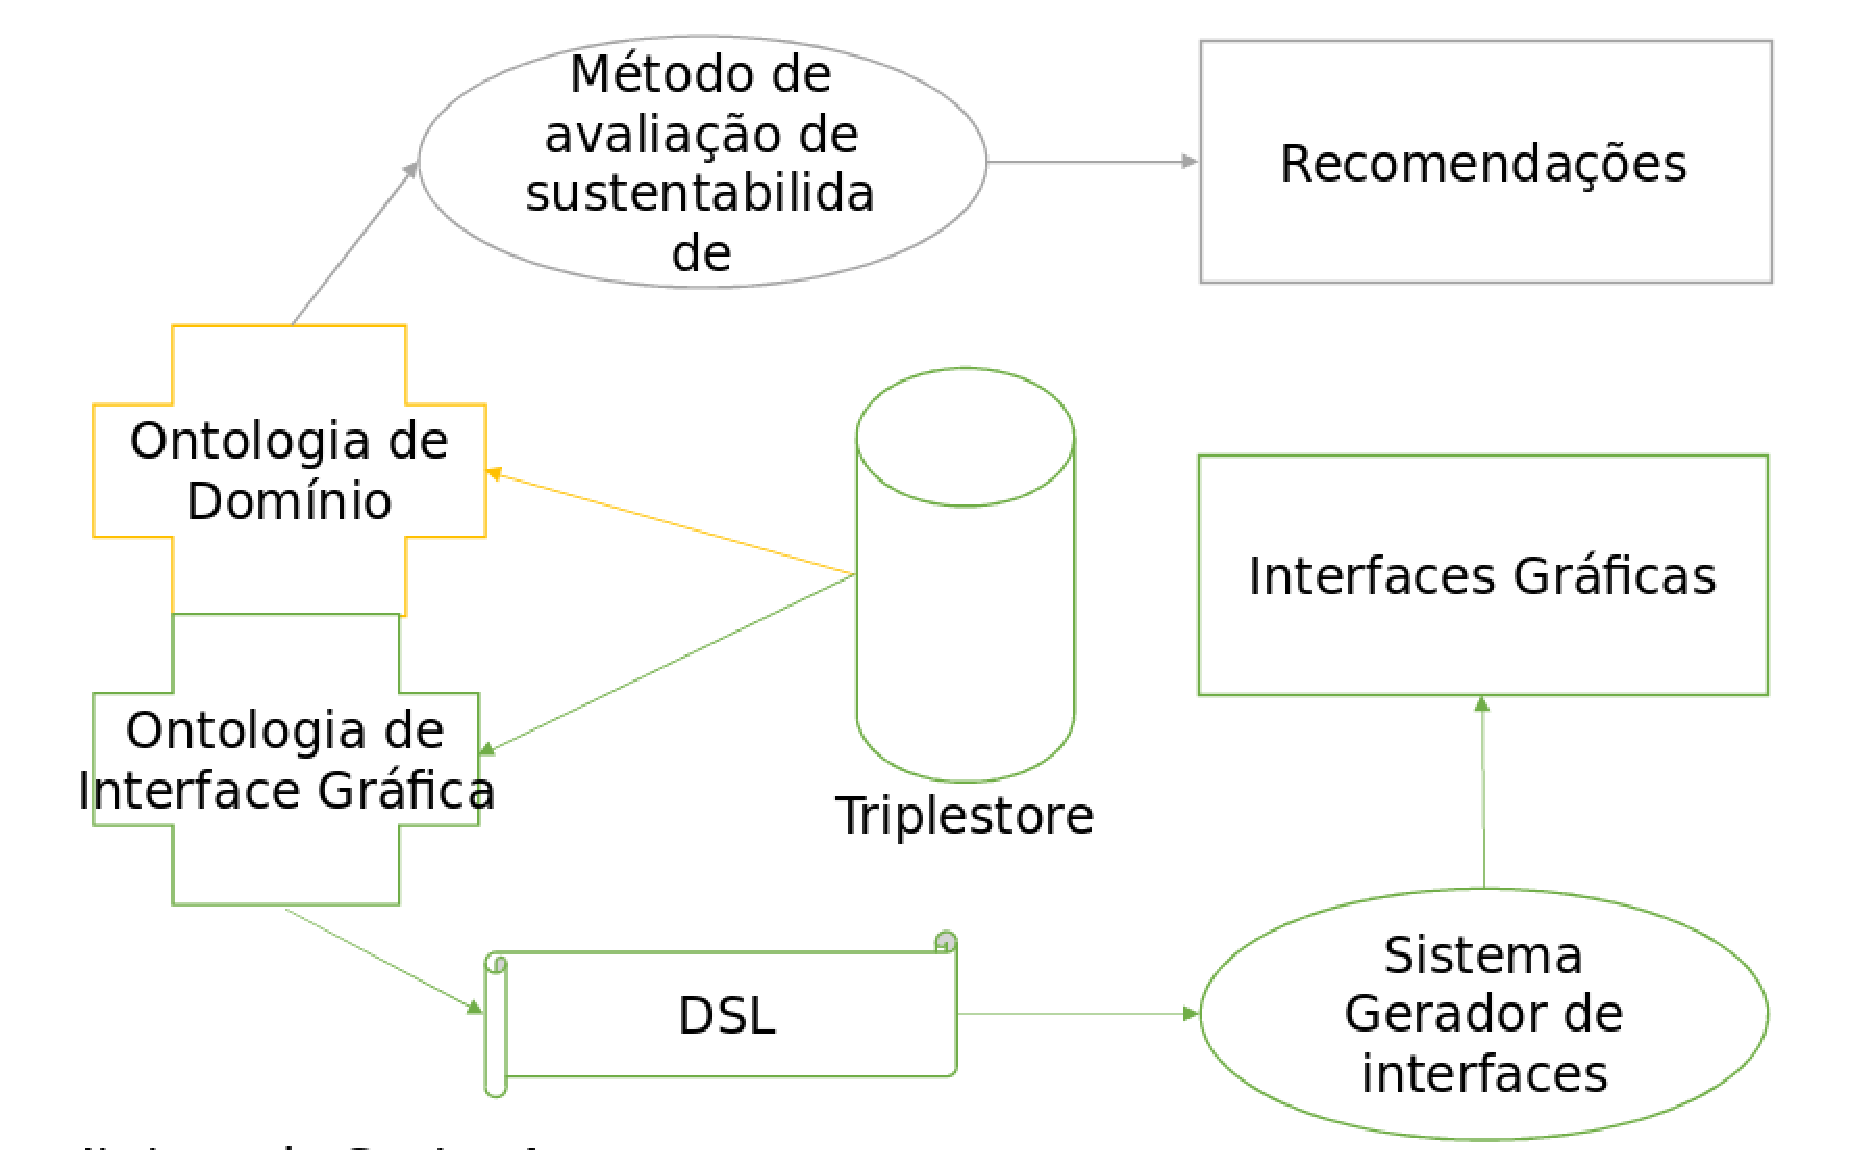
\includegraphics[width=0.9\columnwidth]{../figures/arquitectura}
\par\end{centering}
\centering{}\caption{Arquitetura de SustenAgro \label{fig:Architecture}}
\end{figure}

\begin{enumerate}
\item Ontologia do domínio: ontologia que representa os conceitos do domínio:
avaliação da sustentabilidade do sistema produtivo de cana-de-açúcar.
Ela é a base fundamental para o sistema SustenAgro porque permite
estabelecer os conceitos fundamentais são utilizados pelo sistema,
entre eles: indicadores, componentes de indicadores, índices, dimensões
da sustentabilidade, recomendações e o método de avaliação.
\item Ontologia de controles gráficos: ontologia que representará os controles
de usuários e os tipos de dados, fazendo um mapeamento entre os dois.
\item TripleStore: sistema de recuperação da informação que padroniza as
informações em formato de triplas, permitindo a compatibilidade e
o reúso das informações entre fontes de dados externas.
\item DSL: linguagem especifica do domínio dos elementos visuais que serão
usados pelo SustenAgro. Ela permitirá uma definição flexível das interfaces,
baseada nos conceitos definidos na ontologia de domínio e de controles
gráficos. Ela permitirá a definição das características visuais e
dos tipos de controles especializados para cada conceito da ontologia
de domínio.
\item Sistema gerador de interfaces gráficas: Sistema gerador de GUIs para
sistemas Web, que é definido na DSL e na ontologia de controles gráficos.
\end{enumerate}
O desenvolvimento SustenAgro foi realizado com a finalidade de generalizar
os componentes e assim definir o Decisioner para gerar outros SADs
que trabalhem em domínios similares ao SustenAgro. 

O desenvolvimento do SustenAgro será feito usando-se uma DSL baseada
na linguagem Groovy \citet{koenig2007groovy}. Ou seja, essa DSL será
uma extensão da linguagem Groovy. Groovy é uma linguagem que tem suporte
ao desenvolvimento de DSLs. Isso inclui suporte a DSL Descriptors,
arquivos Groovy que descrevem extensões \emph{domain-specific} para
o motor de inferência e assistente de conteúdo do plugin Groovy\nobreakdash-Eclipse.
Isso permite que a DSL criada tenha todo o mesmo suporte que o IDE\nomenclature{IDE}{Integrated Development Environment}
Eclipse dá a linguagens como Java ou Groovy, como code completion,
debugging, etc. Uma outra vantagem de Groovy é a disponibilidade do
Grails Framework para a criação de aplicações Web \citet{judd2008beginning}.
O desenvolvimento dessa DSL será feito em outro trabalho de mestrado.
Mas este trabalho irá contribuir com a parte da DSL que tem haver
com interfaces, além da ontologia de Controles Gráficos.

O uso da DSL por especialistas em sustentabilidade deve diminuir o
esforço necessário para se desenvolver um SAD nesse domínio. Mas mesmo
assim, ainda será necessário aplicar alguma metodologia de desenvolvimento
de software. 

Existem múltiplos métodos e metodologias que permitem um desenvolvimento
ágil de software. Nesse contexto, o termo ágil refere-se ao desenvolvimento
em tempos curtos e geração de protótipos facilmente adaptáveis às
mudanças. Exemplos de métodos ágeis são: “Mockups”, “User Stories”,
“Scenarios”, “Storyboards” e “Use Cases”, exemplos de metodologias
ágeis são: “SCRUM” ou “XP eXtreme Programming”.

Uma das etapas mais importantes dos desenvolvimentos ágeis é o levantamento
de requisitos. Essa etapa tem como objetivo definir as características
do software e pode ser realizada múltiplas vezes. Isso ocorre pois
as metodologias ágeis são cíclicas e os protótipos mudam em cada ciclo
para cumprir os requisitos.

O desenvolvimento do sistema SustenAgro será realizado por meio de
metodologias ágeis de desenvolvimento de software, principalmente
serão utilizadas algumas práticas da metodologia SCRUM \citet{schwaber2002gile}.
Também será usado o enfoque User-Centered Design. Nesse sentido, está
sendo desenvolvido primeiramente um \emph{mockup} da interface gráfica
do sistema, o qual será o meio de comunicação com os parceiros do
SustenAgro para determinar as funcionalidades básicas do sistema.
Quando o \emph{mockup} for validado, será iniciado o desenvolvimento
de um protótipo da interface gráfica que permitirá determinar os requisitos
funcionais.

Baseando-se na DSL, pode-se suportar um sistema gerador de interfaces
gráficas para conceder usabilidade e flexibilidade ao sistema. Essa
última característica constitui uma nova proposta de desenvolvimento
de SADs que permite a adaptação automática (ou semi\nobreakdash-automática)
da interface às mudanças dos conceitos do domínio.

Cada vez que sejam desenvolvidos cada componente de SustenAgro se
realizarão diversos testes para validar as funcionalidades do sistema,
esse processo será realizado com os especialistas para refinar as
funcionalidades do sistema de acordo com os requisitos manifestados.
Espera-se que, usando a DSL, os próprios especialistas vão ser capazes
de fazer parte do desenvolvimento e validação.

\begin{comment}
\begin{enumerate}
\item \textbf{!!Ainda falta mexer com esta parte!!} 
\item Recuperação dos dados dos repositórios FAO Linked Data\nomenclature{FAO Linked Data}{Food and Agriculture Organization of the United Nations (FAO) Linked Data}
e AGRIS referente aos locais que foram realizadas coletas de espécimes

\begin{enumerate}
\item Análise dos dados de baixa qualidade, ou seja, dados que não tem informações
importantes, por exemplo, localidade e município
\item Verificação do número de dados imprecisos e exibição dos mesmos em
um mapa
\item Verificação do número de dados que contém informações sobre local,
latitude, longitude
\item Verificação da quantidade de dados que possuem informações de latitude
e longitude antes e depois do uso de GPS por biólogos em coletas
\end{enumerate}
\item Utilização de dados de fontes externas como Geonames, Wikimapia, DBpedia
\item Implementação de um método para agrupar todos os dados dos repositórios
SpeciesLink e GBIF e realizar a resolução de topônimos utilizando
técnicas de Recuperação de Informação Geográfica e ontologias
\item Aprimoramento das informações geográficas ausentes nos dados do SpeciesLink
e GBIF

\begin{enumerate}
\item Utilização dos dados referente aos repositórios externos para melhorar
os registros das localidades dos repositórios SpeciesLink e GBIF
\item Criação um método para sumarizar as coordenadas geográficas de acordo
com a abordagem da Lei de Linus
\end{enumerate}
\item Verificação da quantidade de dados que tiveram suas informações aprimoradas

\begin{enumerate}
\item Contagem dos dados que não contém informações sobre latitude, longitude
e foram recuperados
\item Contagem dos dados que possui informações geográficas recuperadas
e eram muito velhos, ou seja, antes do uso de GPS por biólogos em
coletas
\item Análise dos resultados dos passos a) e b) anteriores utilizando o
teste t de Student, para verificar o quão boa foi a abordagem utilizada
\end{enumerate}
\item Mapeamento dos dados para uma \textit{triplestore} utilizando ontologias

\begin{enumerate}
\item Definição das triplas em RDF, que deveram possuir um sujeito, predicado
e objeto para cada localidade. 
\item Mapeamento de coordenadas geográficas para GeoSPARQL 
\end{enumerate}
\item Construção de uma base de teste com informações sobre qual consulta
representa uma localidade

\begin{enumerate}
\item Construção de consultas semânticas e verificação de resultados utilizando
as medidas de precisão, revocação e F1 
\item Realização da mesma abordagem do passo a) para os repositórios DBpedia
e Geonames, com intuito de verificar a viabilidade para expansão de
consultas
\end{enumerate}
\item Desenvolvimento de uma interface que permita aos biólogos inserir
dados no \textit{Gazetteer }por meio de mapas

\begin{enumerate}
\item Desenvolvimento de um método que permita aos biólogos inserir lugares
usando GeoTAGS
\item Agrupamento dos dados inseridos e aprimoramento dos dados referentes
a localidades que são similares.
\item Desenvolvimento de um método que permita aos biólogos inserirem links
do DBpedia, quando os mesmos existirem, para auxiliar no crescimento
da \textit{Web of Data}. 
\item Desenvolvimento de um método que permita aos biólogos verificarem
a acurácia dos links sobre a DBpedia inseridos no \textit{Gazetteer} 
\end{enumerate}
\item Verificação do número de lugares inseridos pelos usuários e qualidade
dos dados 

\begin{enumerate}
\item Verificação da média de usuários que concordam com as coordenadas
geográficas
\item Verificação da média de usuários que concordam com as informações
de \emph{Linked Open Data} presentes no \textit{Gazetteer} 
\item Verificação da quantidade de dados que tiveram suas informações aprimoradas
\end{enumerate}
\end{enumerate}
\end{comment}


\section{Metodologia das ontologias}

O conhecimento do domínio envolvido no sistema SustenAgro está em
contínua construção. Por isso, é necessário um enfoque que permita
realizar mudanças na estrutura e no conteúdo usados no sistema durante
seu desenvolvimento. As ontologias permitem representar o conhecimento
de um domínio por meio de formatos, como a linguagem OWL, permitindo
separar o conhecimento das outras partes do sistema.

Os modelos OWL permitem a compilação do conhecimento em sistemas de
armazenamento e recuperação de informação, chamados \foreignlanguage{english}{triple-stores},
que são bancos de dados e que adicionam significado semântico aos
seus dados.

Na Figura \ref{fig:Methodology} é apresentada a proposta metodológica
que guiará o desenvolvimento das ontologias. Ela tem natureza cíclica,
gerando, em cada ciclo, um protótipo funcional.

\begin{figure}[H]
\begin{centering}
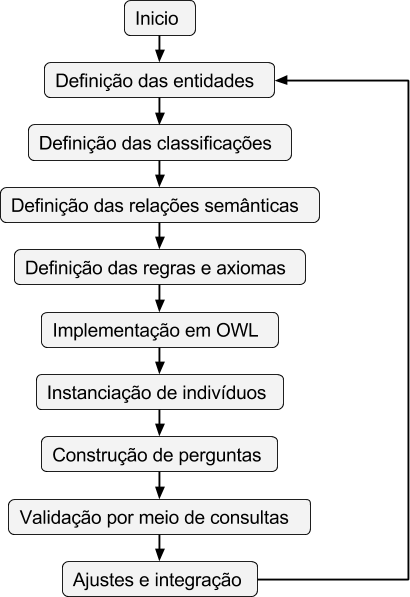
\includegraphics[width=0.6\columnwidth]{../figures/fluxograma}
\par\end{centering}
\caption{Metodologia de definição das ontologias\label{fig:Methodology}}
\end{figure}


\section{Ontologia SustenAgro: avaliação da sustentabilidade}

A ontologia SustenAgro representa o conhecimento base para realizar
uma avaliação de sustentabilidade, está composta de várias classes
fundamentais como \textit{Production Unit, Indicator, Variable, Value,
Microregion}, etc. As quais são integradas e relacionadas para representar
o domínio de avaliação de sustentabilidade em cana-de-açúcar, a continuação
são apresentados as principais classes desta ontologia:

A classe \textit{Production Unit}, representa as organizações que
podem ser avaliadas pelo sistema SustenAgro para obter uma medida
da sustentabilidade, atualmente podem ser \textit{Fornecedores de
cana-de-açúcar} e / ou \textit{Usinas processadoras de cana-de-açúcar},
cada processo de avaliação requer dados que definem as unidades produtivas
através das propriedades que os conformam, existe um conjunto de propriedades
obrigatórias como: 
\begin{itemize}
\item Name: define o nome da unidade produtiva
\item Harvest year: define o ano da safra.
\item Agricultural production system: relaciona o sistema de produção agrícola
em avaliação. 
\item Has microregion: relaciona a microrregião da unidade produtiva 
\item Has state: relaciona o estado Brasileiro 
\item Availability of assessment results: relaciona o tipo de disponibilização
dos resultados. 
\item Sugarcane source: relaciona a origem da cana
\end{itemize}
Na figura \ref{fig:Modelagem-unidade-produtiva} apresenta-se a modelagem
de Production Unit, feita na ferramenta Protégé. 
\begin{figure}[H]
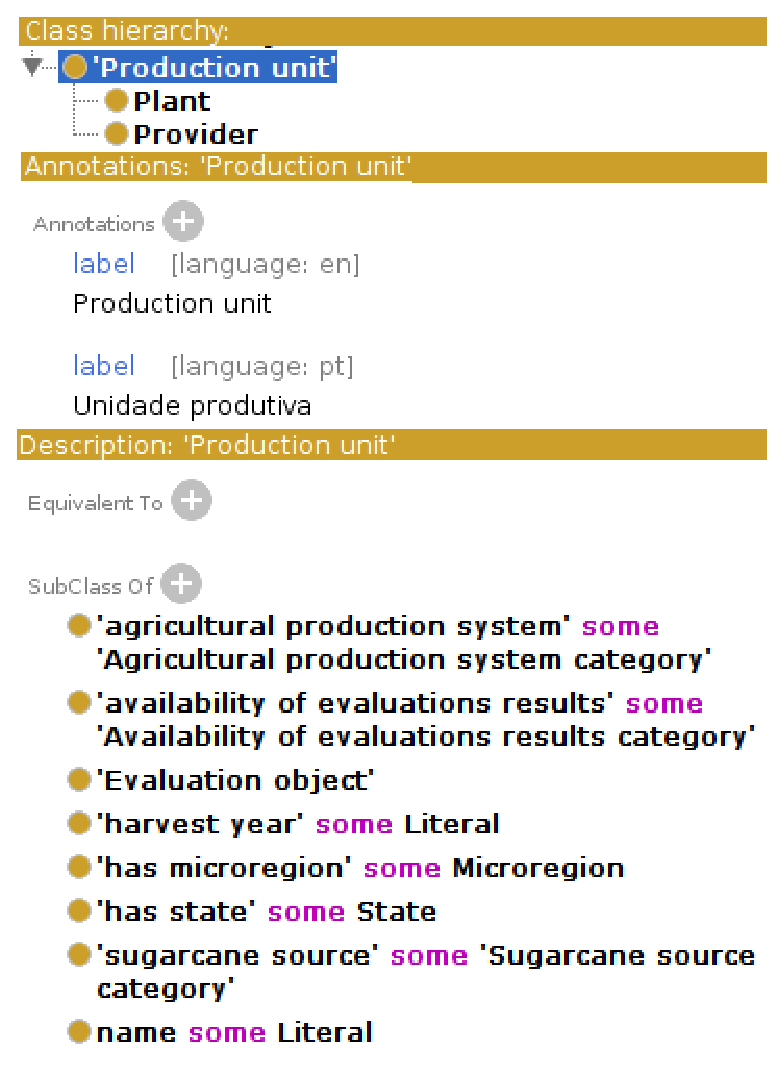
\includegraphics[scale=0.5]{../figures/ProductionUnit}

\caption{Modelagem unidade produtiva \label{fig:Modelagem-unidade-produtiva}}
\end{figure}

As classes \textit{Indicator} e \textit{Variable} representam as características
das unidades produtivas que serão identificadas e quantificadas em
cada processo de avaliação, eles tem um \textit{Value }que os quantifica,
esta propriedade junto com outras conformam um formato que permite
identificar e gerenciar tais elementos.

A figura \ref{fig:Modelagem-de-Indicator} apresenta a modelagem do
indicador \textit{Absolute Emissions Of Greenhouse Gases }que apresenta
a anotação relevance e a propriedade \textit{has value }que estabelece
o formato de um \textit{Indicator}.
\begin{figure}
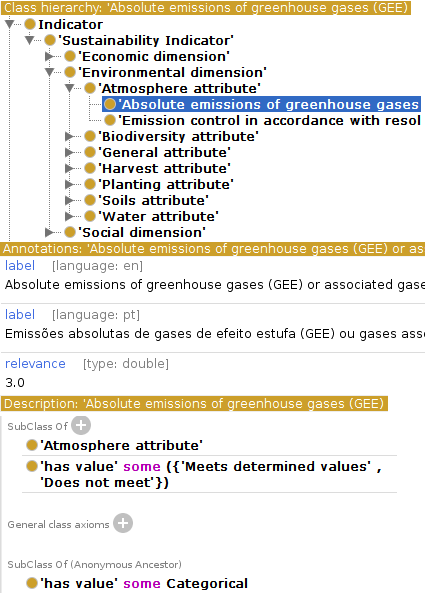
\includegraphics[scale=0.5,bb = 0 0 200 100, draft, type=eps]{/media/john/Data/Master Degree/Dissertation Document/figures/Indicator.png}

\caption{Modelagem de Indicator \label{fig:Modelagem-de-Indicator}}
\end{figure}
A classe \textit{Variable }também representa características das classes
\textit{Production Unit} que permite quantificar-las por meio da propriedade
\textit{has value }e pode ter como opcional um \textit{has weight
}que relaciona um peso por parte do usuário final para atribuir a
importancia de cada característica segundo a \textit{Production Unit}
avaliada.

A figura \ref{fig:Modelagem-de-Var=0000EDavel} apresenta a estrutura
hierarquica das variáveis e a variavel Adequacy of boilers que tem
as duas propriedades descritas anteriormente.

\begin{figure}[H]
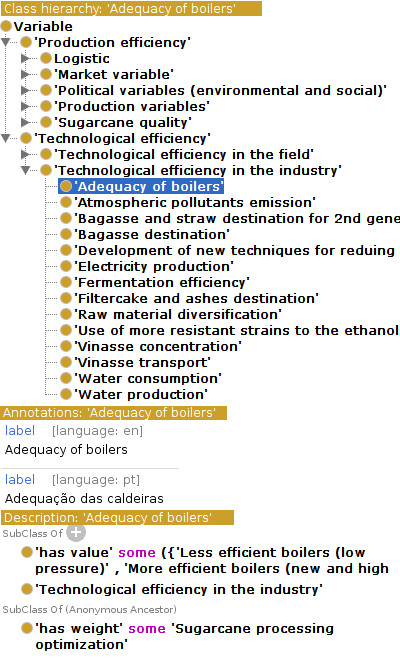
\includegraphics[scale=0.5]{../figures/Variable}

\caption{Modelagem de Variável\label{fig:Modelagem-de-Var=0000EDavel}}
\end{figure}

As classes \textit{State} e \textit{Microregion }representam os lugares
onde são localizadas as unidades produtivas, permitindo definir o
estado e a microrregião para as fazendas e as usinas relacionadas
com cana-de-açúcar, atualmente o sistema SustenAgro tem 7 estados
pertencentes ao centro-sul do Brasil e 243 microrregiões dentro dos
estados registrados, estes dados foram consultados semanticamente
e integrados no sistema a partir de uma consulta na DB-pedia.

A figura \ref{fig:Modelagem-de-Microrregi=0000E3o} representa a modelagem
das localizações geograficas usadas no sistema SustenAgro, com algumas
instancias de \textit{Microregion}.

\begin{figure}[H]
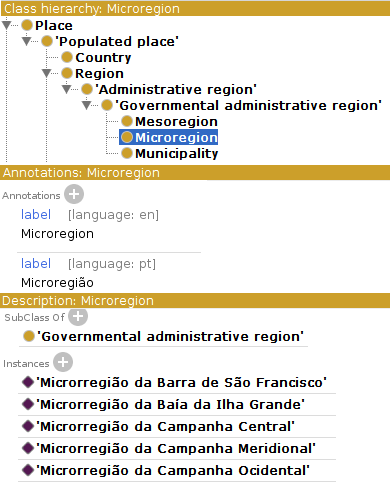
\includegraphics[scale=0.5]{../figures/Microregion}

\caption{Modelagem de Microrregião\label{fig:Modelagem-de-Microrregi=0000E3o}}
\end{figure}

A partir das anteriores classes foi possível desenvolver o modelo
de dados em formato de ontologias da web semântica OWL, as classes
descritas foram relacionados por meio de \textit{Object Properties}
e \textit{Data Properties} que permitem vincular semanticamente as
classes associadas na avaliação de sustentabilidade.

Os \textit{Data/Object Properties} precisam ter definida a propriedade
\textit{rdfs:range }para realizar a validação das classes vinculadas
e algumas são Functional para garantir uma relação de um a um.

\section{Ontologia SAD}

A ontologia de Sistema Apoio à Decisão contem os elementos que foram
abstraidos a partir do analise dos sistemas SAD usados pela Embrapa
Meio Ambiente em seus processos de avaliação.

Os sistemas software de avaliação que foram analisados são:
\begin{enumerate}
\item Sistema SustenAgro: avaliação da sustentabilidade agricola em cana-de-açúcar.
\item Sistema Innova-Tec: avaliação do impacto da inovação tecnológica.
\item Sistema Nano-Tec: avaliação do impacto das nanotecnologias.
\end{enumerate}
A partir desses sistemas foram identificados elementos comuns, que
foram abstraidos na ontologia SAD com o proposito de generalizar as
classes da ontologia sustenagro, para fornecer a geração de interfaces
gráficas .

As classes idenficadas e modeladas são:
\begin{itemize}
\item Evaluation Object: classe que representa os objetos que serão analisados
em cada processo de avaliação, os quais vão ficar como indivíduos
desta classe ou de alguma subclasse dela, no caso do sistema SustenAgro
a classe \textit{Production Unit }é subclasse do Evaluation Object.
\item Feature: classe que representa as caraterísticas de um Evaluation
Object que serão quantificadas, analisadas e usadas no processo de
geração de resultados do processo de avaliação, pelo geral as Features
tem uma propriedade numérica que a quantifica.
\item Analysis: classe que vincula o resultado de uma avaliação, o nome
e data da avaliação, assim como o Evaluation Object, para representar
uma avalição
\item Value: classe que representa os valores que são atribuídos a cada
instancia de Feature.
\item User: classe que representa os usuários do sistema.
\item Role: classe que representa os tipos de usuário do sistema, relacionando
as permissões de cada tipo, por padrao tem estão instanciados os perfis
User e Admin
\end{itemize}
Na figura \ref{fig:Modelagem-do-SAD} é apresentada a modelagem basica
da estrutura de um SAD, com as classes que foram obtidas a partir
da abstração da ontologia SustenAgro.

\begin{figure}[H]
\includegraphics[scale=0.5]{\string"../figures/DSS ontology\string".eps}\caption{Modelagem abstracto do SAD\label{fig:Modelagem-do-SAD}}
\end{figure}

A classe \textit{Value }representa os valores que são relacionados
com cada característica da unidade produtiva, o qual esta subdividido
nas classes \textit{Categorical }ou \textit{Real, }no caso de SustenAgro
representa os possíveis valores que um \textit{Indicator} ou \textit{Variable}
pode ter, os elementos discretos e definidos como os categóricos são
modelados como indivíduos da classe, permitindo assim, restringir
as opções de escolha.

Na figura \ref{fig:Modelagem-de-Value} é apresentado a classe \textit{Value}
e as subclasses modeladas, tanto \textit{Categorical} para conjunto
finito de valores e \textit{Real} para valores numéricos, como exemplo
está a classe \textit{Yes/No} que representa os valores de sim e não,
os quais são modelados como indivíduos de dita classe.

Cada individuo da classe \textit{Value} tem a propriedade \textit{as
number }que relaciona um valor numérico para definir um critério de
comparação e fornecer um formato para este tipo de dados.

\begin{figure}[H]
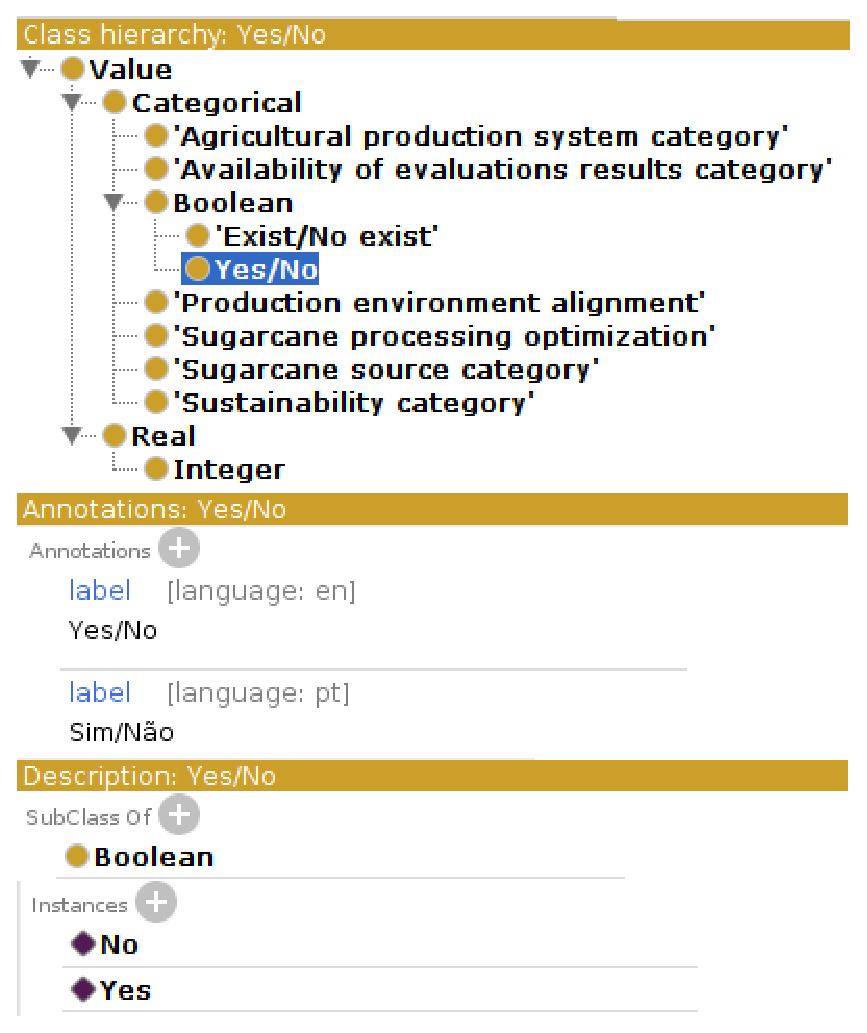
\includegraphics[scale=0.5]{../figures/Value}

\caption{Modelagem de Value\label{fig:Modelagem-de-Value}}
\end{figure}

Estas classes são complementadas com propiedades como rdfs:range ou
por padrões dos dados que relacionam as widgets mais apropriadas na
representação de informações, e assim fornecer a geração de interfaces
graficas de usuário.

A partir do anterior formato a classe 

Para definir a ontologia de domínio do SustenAgro, realizou-se uma
pesquisa das fontes de dados relacionadas com ontologias do domínio
de avaliação de sustentabilidade em sistemas produtivos de cana-de-açúcar.
Concluiu-se que não existem ontologias que suportem esse domínio,
por isso propõe-se desenvolver uma ontologia que utilize os conceitos
de avaliação de sustentabilidade e de sistemas agrícolas. Ela deve
fazer uso da pesquisa realizada por \citet{oliveira:2013} e de algumas
tecnologias fornecidas pela FAO. Essa ontologia terá a finalidade
de fornecer uma base conceitual e tecnológica para suportar o processo
de avaliação de sustentabilidade no sistema produtivo da cana\nobreakdash-de\nobreakdash-açúcar
no estado de São Paulo.

O desenvolvimento dessa ontologia ocorrerá de forma ágil e modular,
por meio de técnicas de prototipação rápida, que serão de âmbito e
complexidade crescente, abrangendo grupos de conceitos relacionados
entre si.

O desenvolvimento da ontologia depende essencialmente da comunicação
entre os especialistas e os modeladores. Foram definidos meios de
comunicação e de representação do conhecimento: reuniões presenciais
e virtuais, e o modelos conceituais que permitem uma visualização
direta do domínio.

Inicialmente, o modelo conceitual vai ser representado por meio de
um mapa conceitual que permitirá a comunicação em um formato reconhecido
por cada um dos profissionais envolvidos no projeto. Esse modelo será
representado em OWL (pelos modeladores) e serão definidas instâncias
para cada uma das classes. Depois disso, o especialista do domínio
construirá perguntas de interesse, com as quais os modeladores definirão
consultas que o sistema deverá responder segundo os resultados esperados,
conseguindo validar e ajustar até ter um protótipo confiável.

Uma das principais contribuições da ontologia é que ela será uma representação
semântica do conhecimento de domínio tanto para os usuários como para
o sistema computacional. Isso evitará problemas de falhas de entendimento
entre os especialistas de domínio e os programadores desenvolvendo
os SADs. A figura \ref{fig:sketch} é um primeiro esboço dos elementos
que serão contidos na ontologia.

\begin{figure}
\begin{centering}
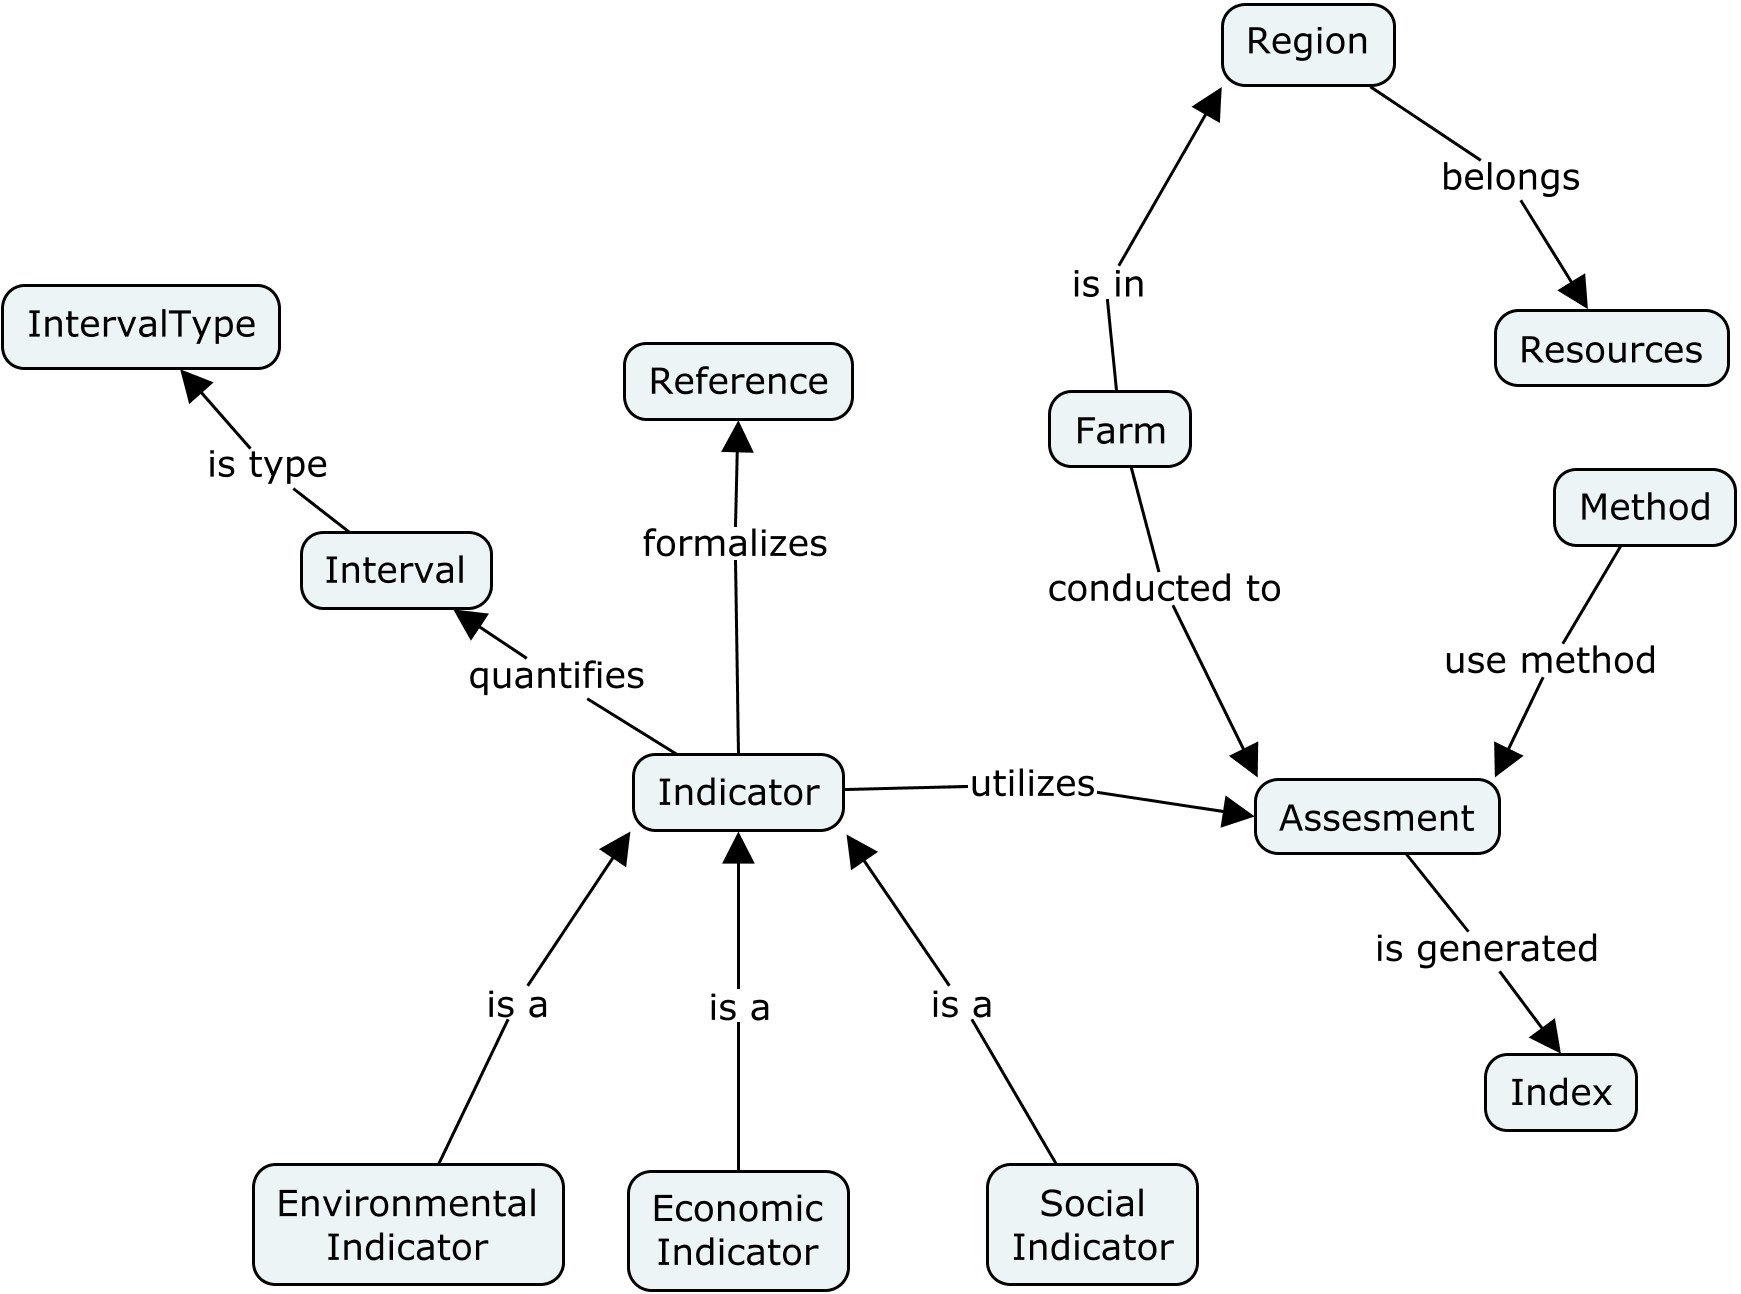
\includegraphics[scale=0.25]{../figures/esboco}
\par\end{centering}
\caption{Primeiro esboço do mapa conceitual\label{fig:sketch}}
\end{figure}

Nessa primeira aproximação, foi identificado o conceito fundamental
da ontologia, os ``indicadores'', que representam e quantificam
os aspectos críticos do sistema produtivo de cana-de-açúcar, mediante
o uso dos ``limiares'', que estabelecem o intervalo dos indicadores,
que, por sua vez, são instanciados com os valores ``Mais sustentável''
ou ``Menos sustentável''.

Outro conceito fundamental é a ``avaliação''. Ela é composta de
um conjunto de ``indicadores'' e de um ``método'', o qual é aplicado
sobre uma ``fazenda'' ou ``usina''. A avaliação gera ``índices''
que são apresentados junto às ``recomendações'' como resultado do
processo de avaliação.

\section{TripleStore}

O sistema SustenAgro será baseado nas tecnologias da web semântica,
entre as tecnologias existentes encontra-se a Triplestore que é um
banco de dados para o armazenamento e recuperação de triplas \citet{rusher2003triple}.
Para o presente projeto foi selecionada a Triplestore Parliament \footnote{http://parliament.semwebcentral.org/}
porque fornece as características: suporte nativo a SPARQL\nomenclature{SPARQL}{SPARQL Protocol and RDF Query Language}
e SPARQL/Update e implementa o SPARQL Protocol Endpoint. Esse último,
padroniza o armazenamento e recuperação da informação; e a compatibilidade
com os sistemas web por meio do Endpoint.

\section{Sistemas de apóio à decisão}

Os sistemas de apóio à decisão (SAD) ajudam no entendimento de processos
complexos, auxiliam na comparação dos fenômenos envolvidos e suportam
a análise e escolha de alternativas no processo de decisão \citep{heinzle2010semantica}.

O sistema SustenAgro é um SAD e será desenvolvido com o apoio da equipe
do projeto SustenAgro (Anexo \ref{chap:Projeto-SustenAgro}) da Embrapa
Meio Ambiente, a qual está desenvolvendo uma proposta metodológica
para avaliar a sustentabilidade de sistemas de produção de cana-de-açúcar
no Centro Sul do Brasil para equacionar as principais questões referentes
a esses sistemas produtivos e possibilitar a utilização racional dos
recursos naturais para suprir as necessidades presentes e garantir
o suprimento das gerações futuras.

A equipe de TI do SustenAgro determinou que o tipo de sistema mais
conveniente para o desenvolvimento seria um Sistema de Apóio à Decisão
(SAD). Com a finalidade de definir a arquitetura e a interface gráfica
desse sistema realizaram-se duas perguntas de pesquisa que orientaram
esse projeto:
\begin{itemize}
\item Como integrar o conhecimento dos especialistas em um sistema de apoio
na tomada de decisões permitindo a continua mudança do modelo do domínio?
\item Como gerar interfaces gráficas a partir de definições simples do domínio
do conhecimento?
\end{itemize}
Tendo em conta os requisitos do software, como o suporte a contínua
mudança do modelo de dados e a geração dinâmica de interfaces, se
propõe a arquitetura a seguir.

\section{Ontologia de avaliação de Sustentabilidade}

O conhecimento sobre sustentabilidade no sistema de produção de cana-de-açúcar
foi representado por meio de entidades, classes, relações semânticas
e axiomas. Ditos elementos constituíram a ontologia, representado
formalmente os conceitos do domínio, os quais foram integrados em
cada uma das funcionalidades do sistema permitindo a personalização
e vinculação da informação para satisfazer os requisitos dos usuários
do sistema SustenAgro.

Eles são sistemas complexos que integram fenômenos de natureza diversa
\citep{simon1991architecture}, integrando três subsistemas: (i) o
subsistema ambiental que fornece as condições físicas, químicas e
biológicas que suportam o desenvolvimento das culturas, (ii) o subsistema
social que integra organizações e pessoas que realizam a produção,
relacionando-se internamente e externamente com os sistemas produtivos
e (iii) o subsistema econômico que estabelece as condiciones de oferta
e demanda dos produtos e subprodutos do sistema de produção agrícola;das
interações entre estes subsistemas, emerge um comportamento complexo
que requer uma abordagem holística e inter-relacionada para suportar
a tomada de decisões que garantam a sustentabilidade do sistema em
analise.

ditos sistemas também são chamados dimensões da sustentabilidade,
segundo a literatura estas dimensões são: ambiental, econômica e social
\citep{AlkanOlsson:2009}.

O software SustenAgro baseou-se em indicadores da sustentabilidade
nas tres dimensões, os quais foram propostos por um grupo de especialistas
de diversas áreas da produção agrícola e sustentabilidade \citep{oliveira:2013},
esta base conceitual foi padronizada por meio de ontologias para representar
e organizar dito conhecimento, conseguindo assim uma representação
compreensível pelos humanos e computadores \citep{allemang2011semantic},
além de fornecer suporte com outras tecnologias da web semântica e
assim realizar consultas complexas que permitam responder perguntas
de interesse para os usuários do sistema software.

O conhecimento sobre sustentabilidade no sistema de produção de cana-de-açúcar
foi representado por meio de entidades, classes, relações semânticas
e axiomas. Ditos elementos constituíram a ontologia, representado
formalmente os conceitos do domínio, os quais foram integrados em
cada uma das funcionalidades do sistema permitindo a personalização
e vinculação da informação para satisfazer os requisitos dos usuários
do sistema SustenAgro.

O desenvolvimento da Ontologia de Domínio do SustenAgro foi iniciado
com a criação de um mapa conceitual entre um grupo de especialistas
em modelagem de conhecimento. Na reunião da equipe na Embrapa Informática
Agropecuária (UNICAMP - Campinas), foram identificados os principais
conceitos em cada uma das dimensões da sustentabilidade: ambiental,
social e econômica. 

O sistemas agricolas foram modelados por meio de três subsistemas:
(i) o subsistema ambiental que fornece as condições físicas, químicas
e biológicas que suportam o desenvolvimento das culturas, (ii) o subsistema
social que integra organizações e pessoas que realizam a produção,
relacionando-se internamente e externamente com os sistemas produtivos
e (iii) o subsistema econômico que estabelece as condiciones de oferta
e demanda dos produtos e subprodutos do sistema de produção agrícola;
das interações entre estes subsistemas, emerge um comportamento complexo
que requer uma abordagem holística e inter-relacionada para suportar
a tomada de decisões que garantam a sustentabilidade do sistema em
analise.

Cada uma das dimensões faz a função de \emph{container}. Neles estão
contidos os indicadores que foram validados como os mais relevantes
para as condições gerais das fazendas e usinas produtoras de cana-de-açúcar
no estado de São Paulo. Os indicadores têm uma relação de \emph{contains}
com os atributos e uma relação de \emph{considers} com os componentes
dos indicadores.

As três dimensões da sustentabilidade têm uma participação equitativa
no método de avaliação \citep{kraines2011system}. A Figura \ref{fig:environment}
representa a dimensão ambiental, modelo onde são definidos os seguintes
conceitos (\emph{containers}):

\begin{figure}
\begin{centering}
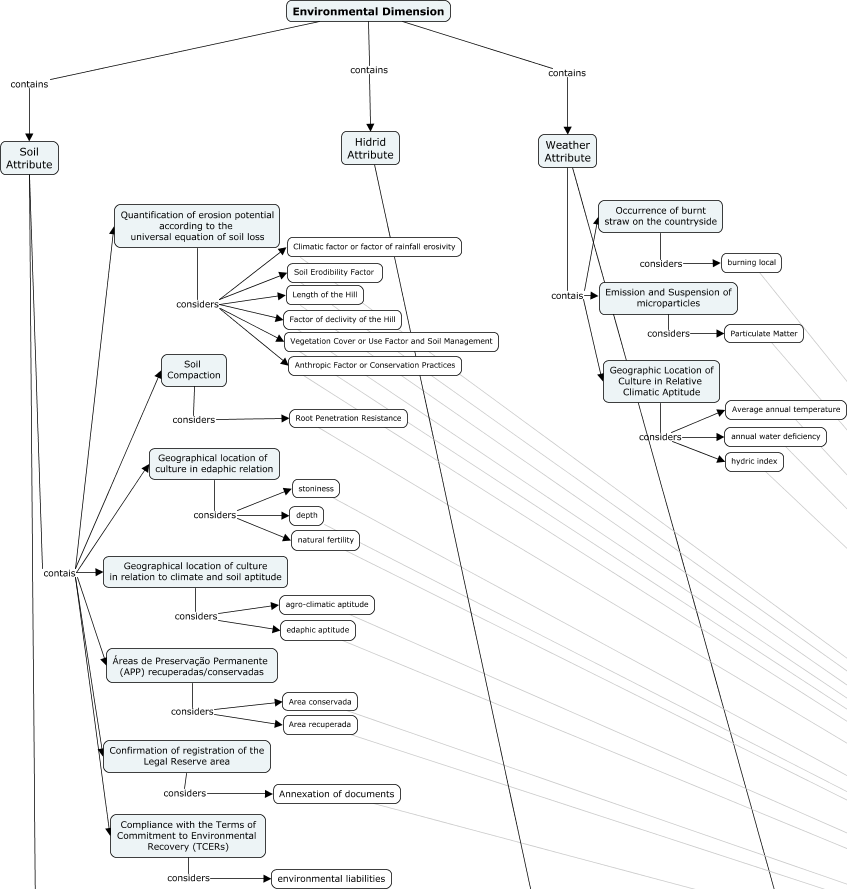
\includegraphics[width=1\textwidth]{../figures/ambiental}
\par\end{centering}
\caption{Mapa conceitual - Ambiental\label{fig:environment}}
\end{figure}

\begin{itemize}
\item Atributo solo: indicadores que avaliam os aspectos referentes às características
do solo.
\item Atributo hídrico: indicadores que avaliam os aspectos referentes à
disponibilidade e qualidade das fontes hídricas.
\item Atributo clima: indicadores que avaliam os aspectos climáticos.
\end{itemize}
Nesta dimensão (ambiental), não foi possível identificar indicadores
de tipo hídrico porque não existe consenso entre os especialistas
consultados sobre quais são os aspectos mais relevantes destes para
a avaliação da sustentabilidade, mas é um aspecto fundamental para
trabalhar nas próximas etapas de pesquisa.

A Figura \ref{fig:social}, representa a dimensão social, onde são
definidos os seguintes conceitos (\emph{containers}):

\begin{figure}
\centering{}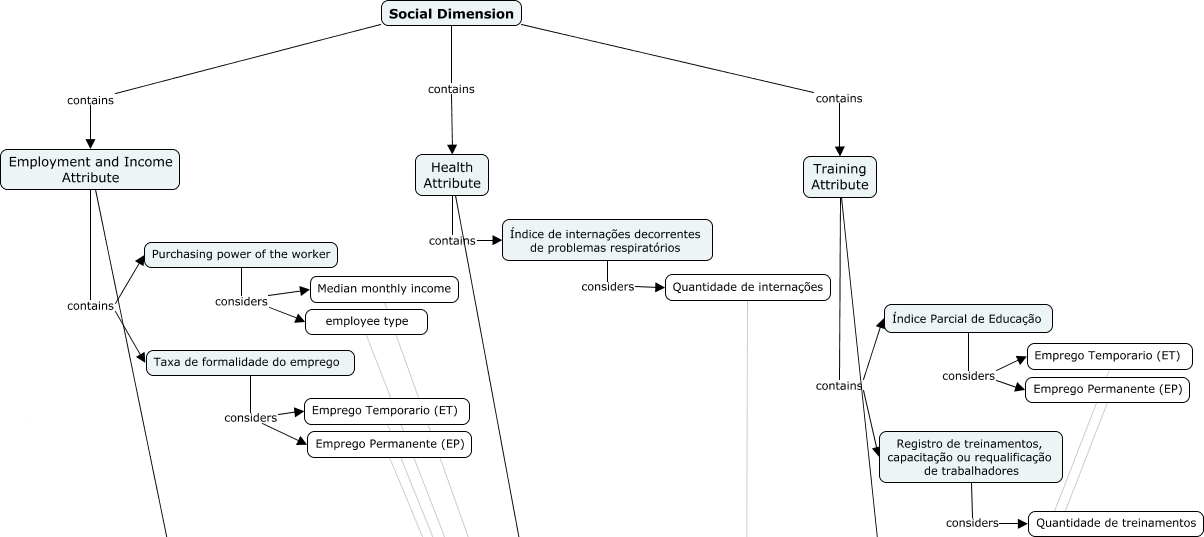
\includegraphics[width=1\textwidth]{../figures/social}\caption{Mapa conceitual - Social\label{fig:social}}
\end{figure}

\begin{itemize}
\item Atributo emprego e renda: indicadores que avaliam os aspectos referentes
à mão-de-obra.
\item Atributo saúde: indicadores que avaliam os aspectos de segurança dos
trabalhadores.
\item Atributo treinamento: indicadores que avaliam os aspectos da capacitação
dos trabalhadores.
\end{itemize}
Nesta dimensão (Social), é importante reconhecer que as unidades produtivas,
sejam do tipo fazendas ou usinas, são compostas por pessoas tanto
internamente como externamente. Por isso, é importante refinar os
indicadores para incluir a população externa à unidade produtiva que
é afetada pelas práticas produtivas.

As Figuras \ref{fig:Economic-1} e \ref{fig:Economic-2} apresentam
a dimensão econômica, onde foram definidos os seguintes conceitos
(\emph{containers}):

\begin{figure}
\begin{centering}
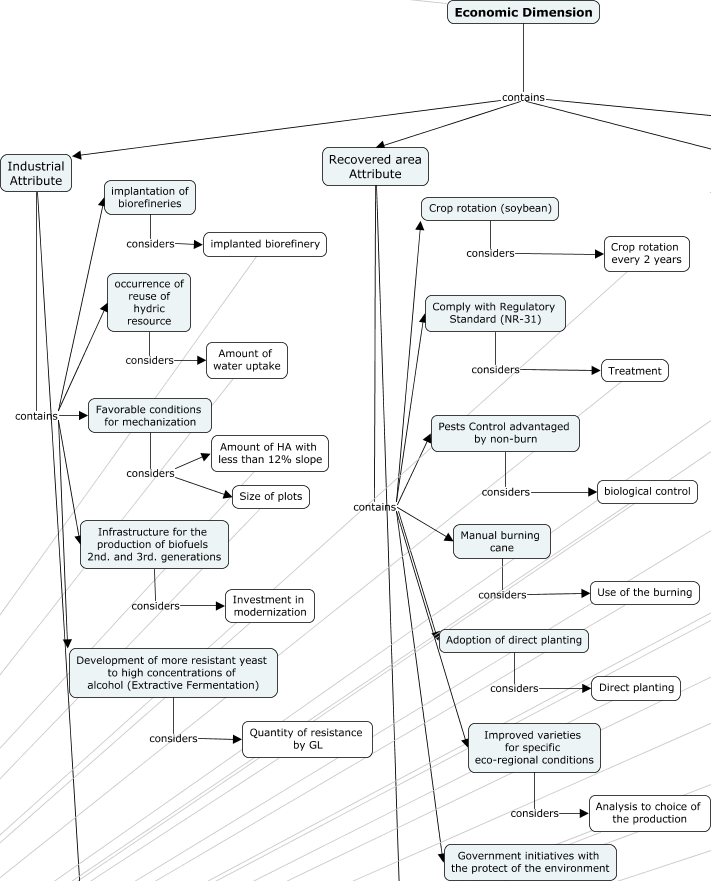
\includegraphics[width=1\textwidth]{../figures/economica_1}
\par\end{centering}
\caption{Mapa conceitual - Dimensão Econômica primeira parte.\label{fig:Economic-1}}
\end{figure}

\begin{figure}
\begin{centering}
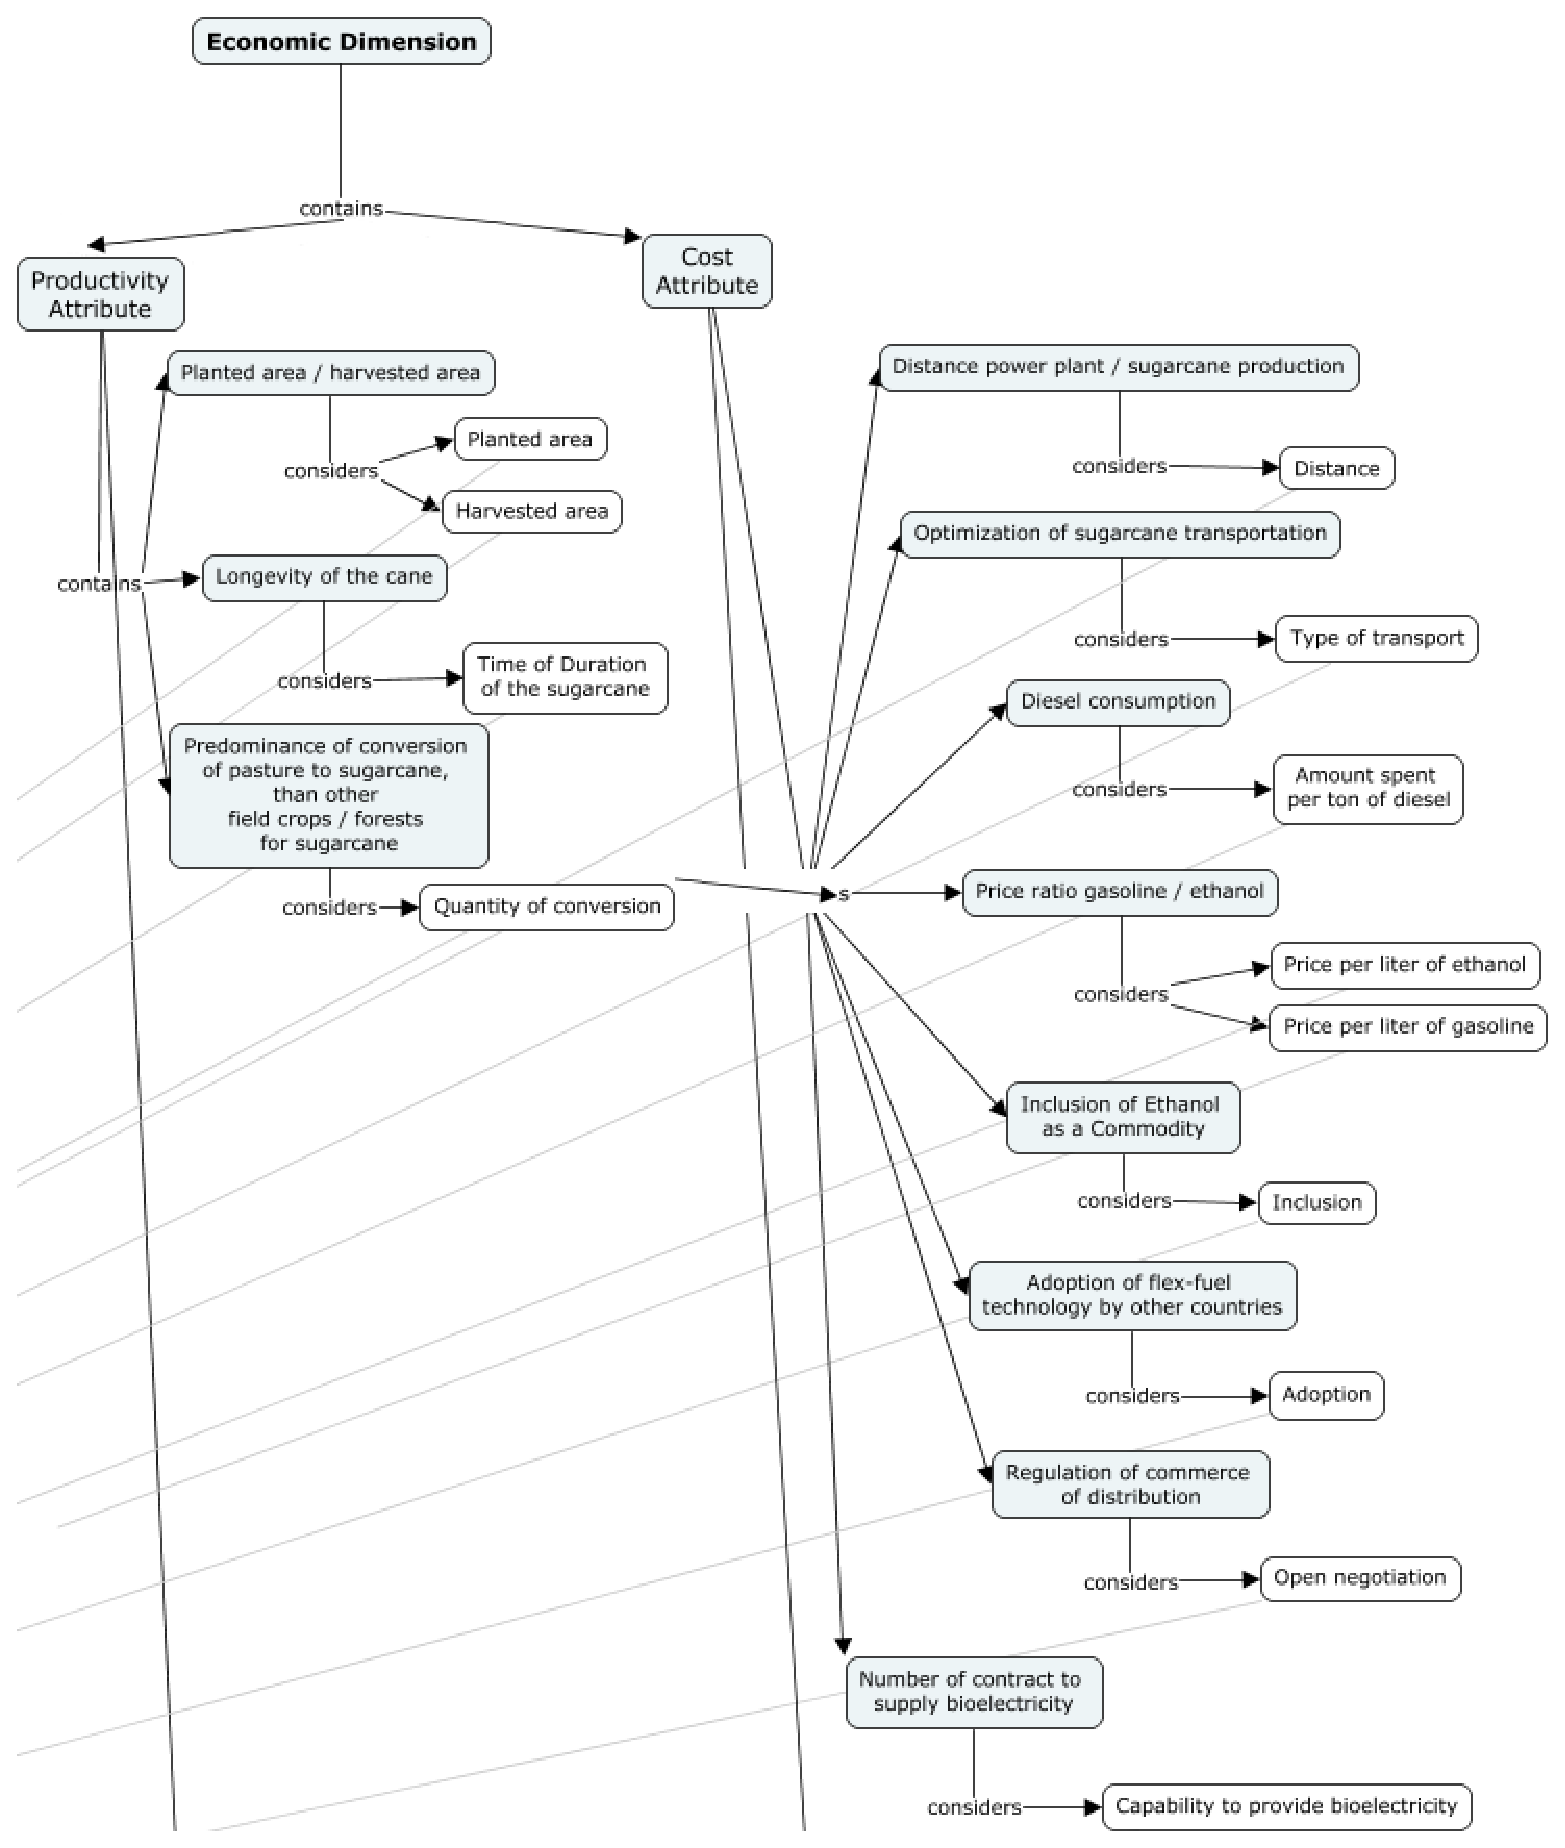
\includegraphics[width=1\textwidth]{../figures/economica_2}
\par\end{centering}
\caption{Mapa conceitual - Dimensão Econômica segunda parte.\label{fig:Economic-2}}
\end{figure}

\begin{itemize}
\item Atributo industrial: indicadores que avaliam os aspectos industriais. 
\item Atributo área recuperada: indicadores que avaliam os aspectos da área
produtiva e das técnicas produtivas.
\item Atributo produtividade: indicadores que avaliam os aspectos dos produtos
e dos processos produtivos.
\item Atributo custo: indicadores que avaliam os aspectos dos custos da
produção. 
\end{itemize}
Cada uma das três dimensões devem ser avaliadas equitativamente para
gerar um resultado coerente com a teoria da sustentabilidade agrícola.

A Figura \ref{fig:Method} mostra os conceitos que fazem a união das
dimensões e do método de avaliação. Cada um dos conceitos relacionados
com o método de avaliação utilizam os indicadores para realizar o
processo de avaliação. A intenção é representar o mais detalhadamente
e claramente possível o processo de avaliação para a sus correta execução.

\begin{figure}
\begin{centering}
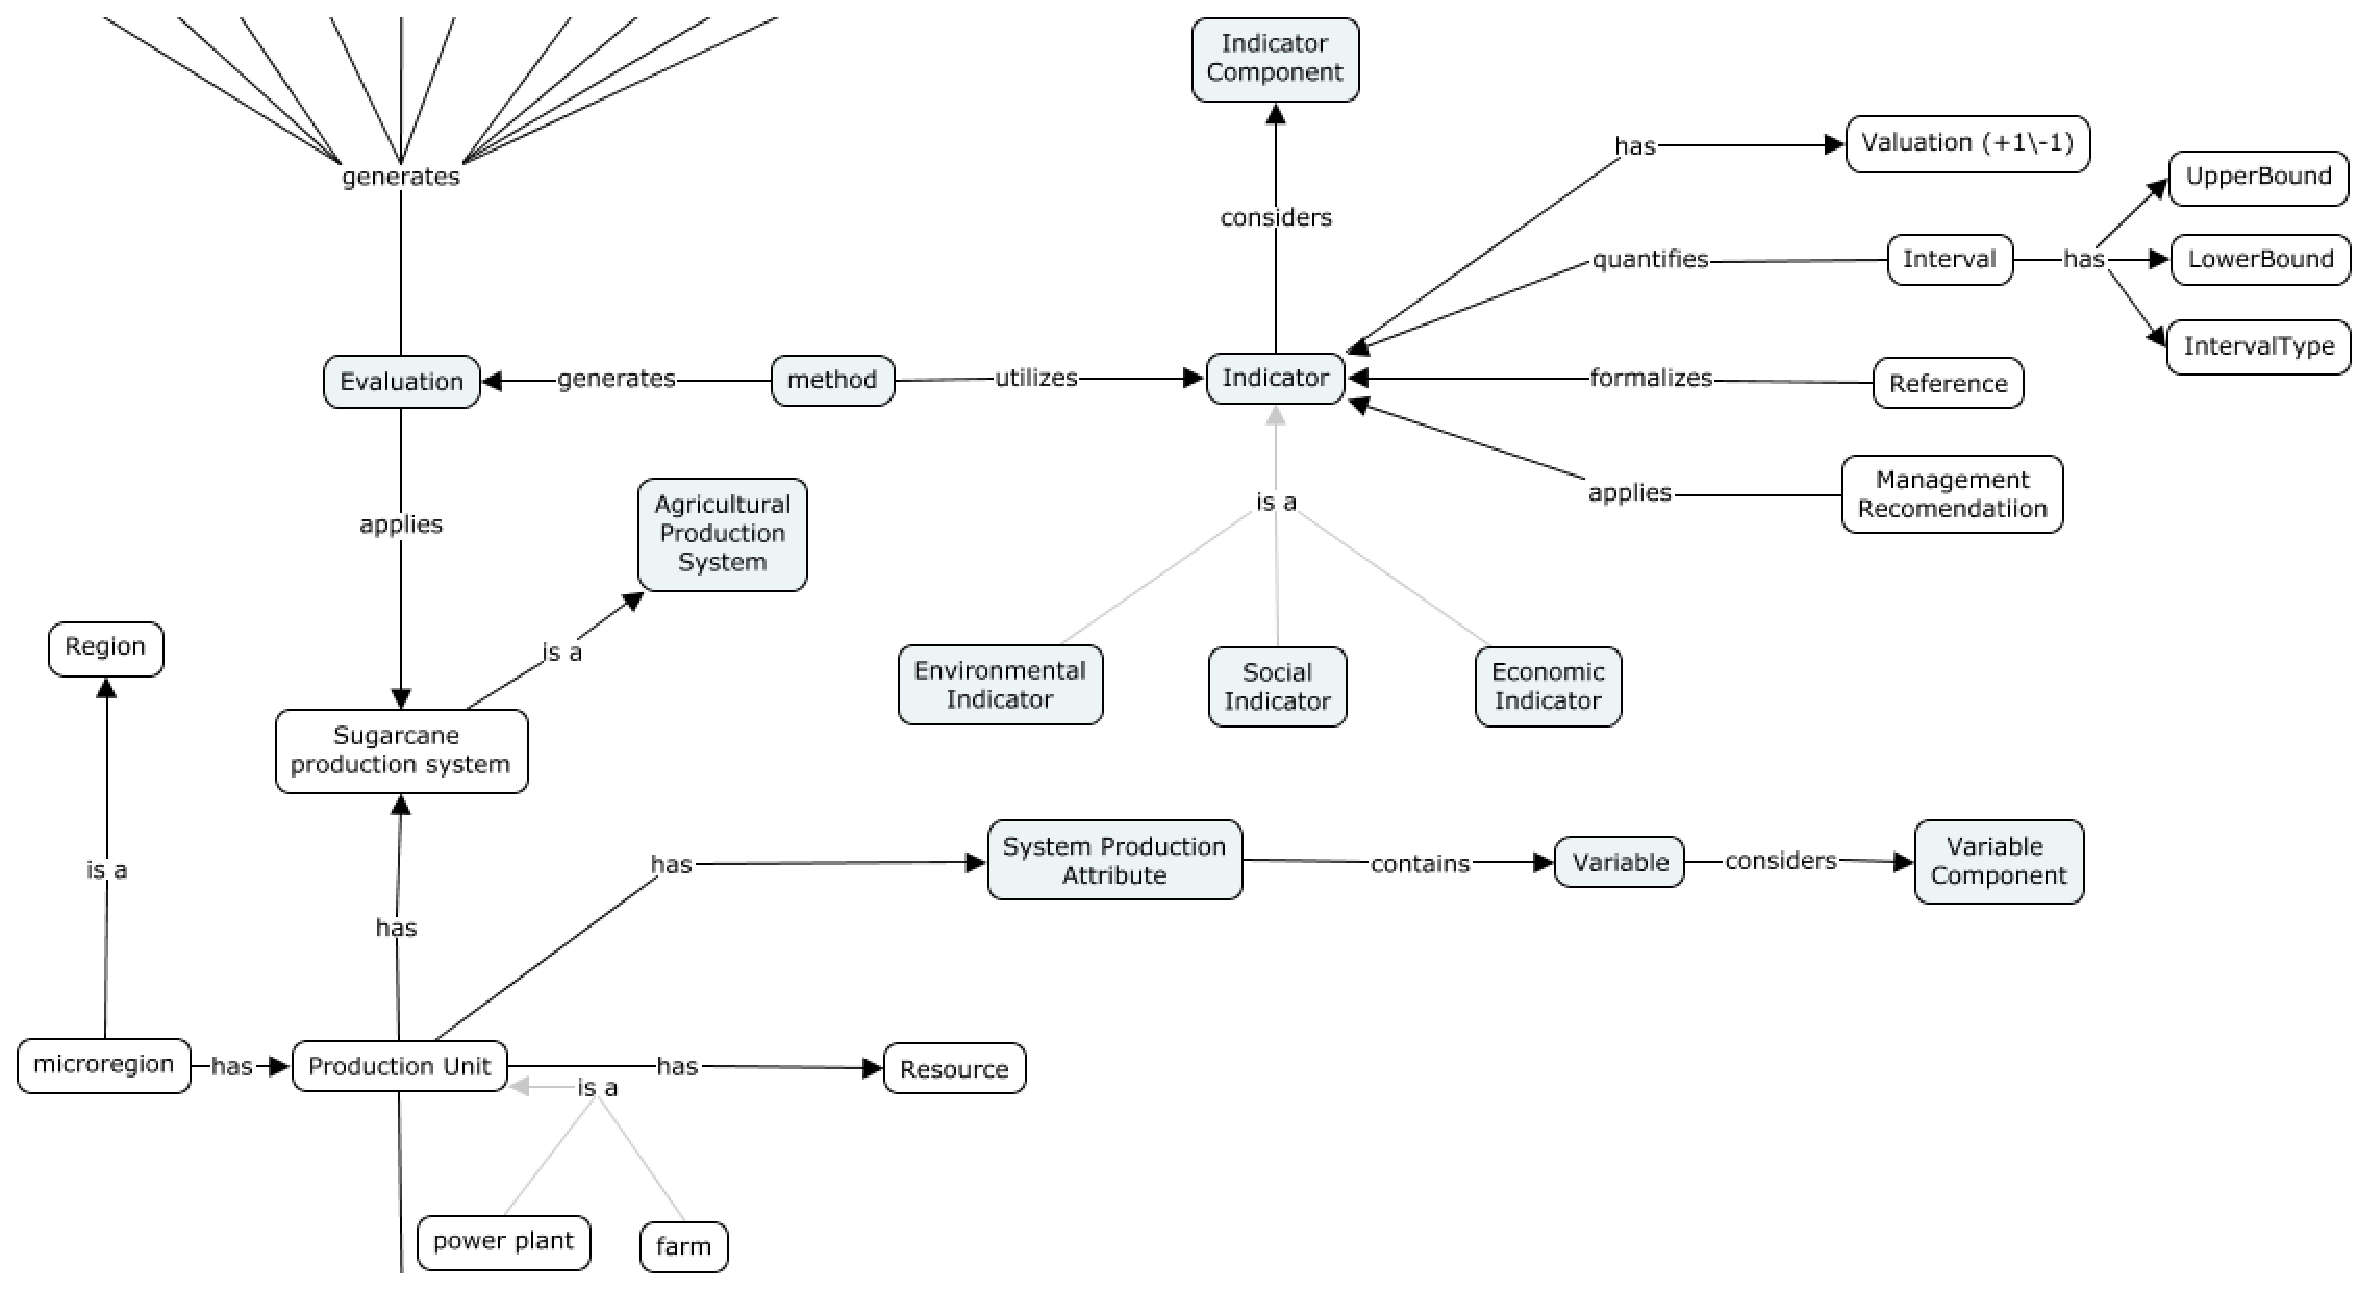
\includegraphics[width=1\textwidth]{../figures/metodo}
\par\end{centering}
\caption{Mapa conceitual - Método\label{fig:Method}}
\end{figure}


\section{User Stories}

Histórias de usuário são uma técnica para descrever, de uma forma
curta e simples, as características do sistema a partir da perspectiva
do usuário ou cliente do sistema, gerando uma definição de alto nível
de um requisito. Seu padrão é: Como um “tipo de usuário”, eu quero
“algum objetivo” para “alguma finalidade”.

Na aplicação dessa técnica foram obtidos as seguintes histórias:
\begin{enumerate}
\item O usuário poderá identificar e cadastrar a localização geográfica
e a área da sua lavoura (definir região geográfica do IBGE, latitude
e longitude - a partir do Google Maps). 
\item O usuário poderá identificar e cadastrar a microrregião a que pertence
a sua lavoura. O sistema fará uma sugestão de cadastro a partir dos
dados da localização geográfica.
\item O usuário deverá preencher o estado de cada indicador específico nas
dimensões ambiental, econômica e social. Esses indicadores vão ser
definidos pelo programa. Eles devem se adaptar às condições das regiões
e microrregiões do Brasil. Da mesma forma as faixas de limiares de
sustentabilidade são definidas.
\item Permitir o emprego da metodologia para avaliação caso a caso: possibilitar
que o usuário selecione quais indicadores vai utilizar. Dentro dos
indicadores, ele pode recomendar limiares mais adequados para a sua
realidade. Ele também pode inserir novos indicadores / limiares.
\item O usuário poderá obter o resultado dos índices segundo a informação
preenchida e a formula de agregação dos indicadores.
\item O usuário poderá armazenar a informação dos indicadores para futuras
consultas.
\item O usuário poderá acrescentar indicadores que considere importantes
para sua análise. Devem-se estabelecer regras para essa funcionalidade
de tal modo que os novos indicadores (criados pelos usuários) sejam
recuperáveis de um modo separado dos indicadores cadastrados no sistema. 
\item Cronograma de avaliação, melhor depois de cada safra. 
\end{enumerate}
O usuário deverá ser informado da importância dos processos de avaliação,
exemplo: 
\begin{itemize}
\item “A crescente demanda de países desenvolvidos por produtos com garantia
de origem tem induzido aumento das certificações nas usinas no Brasil
(ALVES et al., 2008).” 
\item A certificação tem sido uma importante forma de diferenciação de commodities
agrícolas, facilitando seu acesso aos mercados protegidos dos países
desenvolvidos. 
\item A caracterização climática aliada aos detalhes de fertilidade e manejo
do solo (quantificação edafoclimática) são essenciais para a determinação
das regiões aptas ao cultivo de culturas de interesse comercial (CIIAGRO,
2009). 
\end{itemize}
Depois do ingresso da informação sobre os indicadores, o usuário receberá
recomendações classificadas sobre práticas de sustentabilidade recomendadas
com sua argumentação, exemplo: 
\begin{itemize}
\item (Ambiental) “O sistema de plantio direto da cana-de-açúcar sobre leguminosas
proporciona maiores teores foliares de N e K na cana do que o plantio
convencional (JÚNIOR; COELHO, 2008)”.
\item (Ambiental) Segundo Leme (2005), haveria redução de 36\% na emissão
de gases do efeito estufa (GEE) se a palha fosse queimada nas caldeiras
das usinas e destilarias, ao invés de ser queimada no campo.
\item (Ambiental) A queima da cana aumenta a erosão do solo e a poluição
do ar e reduz a qualidade da matéria-prima (LINS; SAAVEDR, 2007). 
\item (Ambiental) Quando a cana não é queimada, proliferam, nos canaviais,
roedores silvestres originários de fragmentos florestais. Esses roedores
podem transmitir o Hantavírus através da urina e contaminar cortadores
de cana, causando uma síndrome respiratória e cardíaca, a pneumocitose,
podendo levar à morte. 
\item (Ambiental) Quando não há queima da cana é comum, também, o aumento
do ataque de cigarrinhas, com perdas significativas de produção (ANDRADE;
DINIZ, 2007). 
\item (Econômico) A utilização das colheitadeiras reverte-se em aumento
da produtividade e da qualidade da matéria-prima, bem como em diminuição
dos custos da produção agrícola, que representam entre 50\% e 60\%
em relação ao custo total (SCOPINHO, 1995).
\item (Econômico e Social) A utilização das colheitadeiras em cooperativa
possibilita a soma das áreas de produtores próximos possibilitando
a mecanização em propriedades com restrição para mecanização.
\item (Econômico) Restrições físicas da propriedade (menos de 500 ha de
área com declividade inferior a 12\% e talhões menores que 800 metros)
dificultam a mecanização. 
\end{itemize}

\section{Scenarios}

É uma técnica que permite a descrição das funcionalidades do sistema
da perspectiva do usuário ou cliente com a descrição detalhada da
interação destes. Em geral, é uma descrição detalhada de cada um dos
passos dos usuários no sistema para alcançar seu objetivo. Abaixo,
serão apresentadas as 8 histórias de usuários do projeto SustenAgro
com os cenários associados a elas:

\textbf{História de usuário \#1:} “O usuário poderá identificar e
cadastrar a localização geográfica e a área da sua lavoura (definir
região geográfica do IBGE, latitude e longitude - a partir do Google
Maps).”
\begin{enumerate}
\item O usuário ingressa na sua conta, através do sistema web SustenAgro
em \url{http://sustenagro.embrapa.br}, e o sistema apresenta a tela
“Home” 
\item O usuário seleciona a aba “lavouras” e dá um click em ``cadastrar
lavoura''. O sistema apresenta a tela de cadastro de lavouras, onde
tem um mapa do Google Maps 
\item O usuário seleciona no mapa um ponto que identificará a localização
da lavoura. Se ele quiser, também é possível marcar a área da lavoura
para que o sistema possa ter dados mais específicos para o processo
de avaliação de sustentabilidade. Uma vez terminado, o usuário dá
um click no botão “seguinte” e o sistema cadastra a informação preenchida. 
\end{enumerate}
\textbf{História de usuário \#2}: “O usuário poderá identificar e
cadastrar a microrregião a que pertence a sua lavoura por meio de
uma sugestão que o sistema faz com os dados da localização geográfica.”
\begin{enumerate}
\item O usuário poderá fazer a “Historia de usuário \#1” ou entrar no sistema
e continuar com o cadastro da lavoura de onde ele tenha parado. O
sistema apresentará uma tela com sugestões de microrregiões. 
\item O usuário poderá escolher a microrregião onde esteja localizada a
lavoura e salvá-la no sistema por meio do botão ``seguinte''. 
\end{enumerate}
\textbf{História de usuário \#3:} “O usuário deverá preencher o estado
de cada indicador específico nas dimensões ambiental, econômica e
social. Esses indicadores vão ser definidos pelo programa. Eles devem
se adaptar às condições das regiões e microrregiões do Brasil. Da
mesma forma as faixas de limiares de sustentabilidade são definidas.''
\begin{enumerate}
\item O usuário poderá fazer a “História de usuário \#2” ou entrar no sistema
e continuar com o cadastro dos indicadores de onde ele tenha parado.
O sistema apresentará uma tela com três abas que contém os controles
que permitiram fazer o cadastro dos indicadores nas dimensões ambiental,
econômica e social. 
\item O usuário dá um click na primeira aba e começa a preencher os dados
dos indicadores ambientais, principalmente os limiares que identificam
o estado do indicador. A interface também permite eliminar ou acrescentar
indicadores específicos por parte dos usuários (funcionalidade que
é explicada na “história de usuário \#4”). 
\item O usuário preenche os dados das outras duas dimensões e o sistema
salva as mudanças.
\end{enumerate}
\textbf{História de usuário \#4:} “Permitir o emprego da metodologia
para avaliação caso a caso: possibilitar que o usuário selecione quais
indicadores vai utilizar. Dentro dos indicadores, ele pode recomendar
limiares mais adequados para a sua realidade. Ele também pode inserir
novos indicadores\slash{}limiares.”
\begin{enumerate}
\item O usuário poderá fazer a “Historia de usuário \#3” ou entrar no sistema
e continuar na tela de cadastro de indicadores e, quando aconteça
que o usuário precise de um indicador que não seja oferecido pelo
sistema, o usuário poderá acrescentá-lo por meio do botão “acrescentar
indicador” 
\item O usuário da click no botão “acrescentar indicador” e lhe é apresentada
uma interface de entrada, onde ele deverá cadastrar o título, a descrição,
os limiares, a medida do manejo e a justificativa desse indicador.
Depois, preenche o estado do indicador e o sistema salva esses dados
nessa dimensão. 
\item O usuário também poderá eliminar alguns indicadores segundo seu critério.
\end{enumerate}
\textbf{História de usuário \#5:} \textquotedbl{}O usuário poderá
obter o resultado dos índices segundo a informação preenchida e a
formula de agregação dos indicadores.\textquotedbl{}
\begin{enumerate}
\item Depois de terminada a “História de usuário \#4”, o sistema fará a
aplicação da metodologia de avaliação, que vai estar definida no sistema
pelos administradores. 
\item O resultado da avaliação vai ser cadastrado no sistema com informações
sobre a metodologia utilizada.
\item A metodologia de avaliação pode ser atualizada pelos administradores
para ser utilizada em avaliações futuras.
\end{enumerate}
\textbf{História de usuário \#6:} ``O usuário poderá armazenar a
informação dos indicadores para futuras consultas.''
\begin{enumerate}
\item O usuário faz qualquer tipo de entrada de dados nos formulários do
SustenAgro. 
\item Esses dados vão ser salvos quando o usuário mudar de formulário ou
quando der um click no botão ``seguinte''.
\end{enumerate}
\textbf{História de usuário \#7:} ``O usuário poderá acrescentar
indicadores que considere importantes para sua análise. Devem-se estabelecer
regras para essa funcionalidade de tal modo que os novos indicadores
(criados pelos usuários) sejam recuperáveis de um modo separado dos
indicadores cadastrados no sistema.''
\begin{enumerate}
\item Quando o usuário estiver preenchendo os indicadores gerados pelo sistema,
o sistema fornecerá um conjunto de controles que permitam a inclusão
de um novo indicador. Esse novo indicador vai ser definido pelo próprio
usuário baseado na sua experiência na área. 
\item O sistema armazenará esse novo indicador com uma classificação especial
que permita sua identificação para avaliar sua relevância. 
\item O usuário poderá preencher os dados do novo indicador, para que sejam
inclusos na avaliação de sustentabilidade.
\end{enumerate}
\textbf{História de usuário \#8:} ``Cronograma de avaliação, melhor
depois de cada safra.''
\begin{enumerate}
\item Depois de fazer o cadastro da fazenda e das culturas que são plantadas
nela, o sistema poderá identificar quando termina cada safra, gerando
um alerta para que u usuário faça o processo de avaliação nessa data.
\item O usuário lerá o alerta e poderá fazer o processo de avaliação de
sustentabilidade. 
\end{enumerate}

\section{Storyboard}

Storyboards são similares aos cenários. Elas ilustram a interação
necessária para se atingir um objetivo sem utilizar uma lista de passos,
a interação é visualizada por meio de uma história de quadrinhos.

Esta representação permite se ter uma visão holística da interação
do usuário, com ênfase nos aspectos funcionais da interação e não
nos aspectos da interface de usuário. A seguir, são apresentados os
textos das storyboard dos processos identificados:

\begin{figure}[H]
\begin{centering}
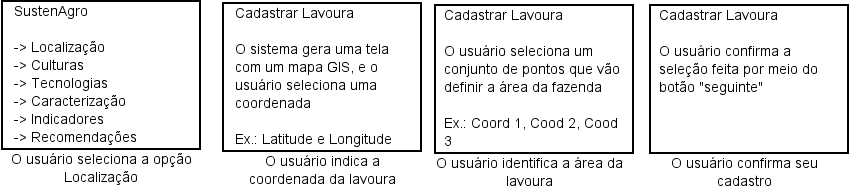
\includegraphics[width=1\columnwidth]{../figures/Story_1}
\par\end{centering}
\begin{centering}
\emph{\small{}StoryBoard 1.}
\par\end{centering}{\small \par}
\smallskip{}

\begin{centering}
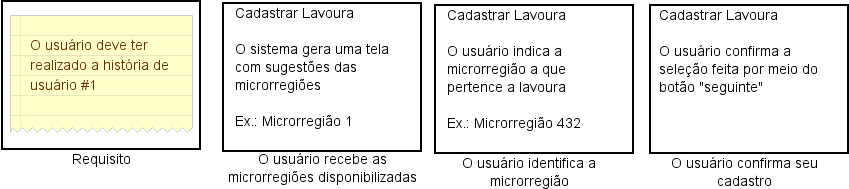
\includegraphics[width=1\columnwidth]{../figures/Story_2}
\par\end{centering}
\begin{centering}
\textit{\small{}StoryBoard 2.}
\par\end{centering}{\small \par}
\smallskip{}

\begin{centering}
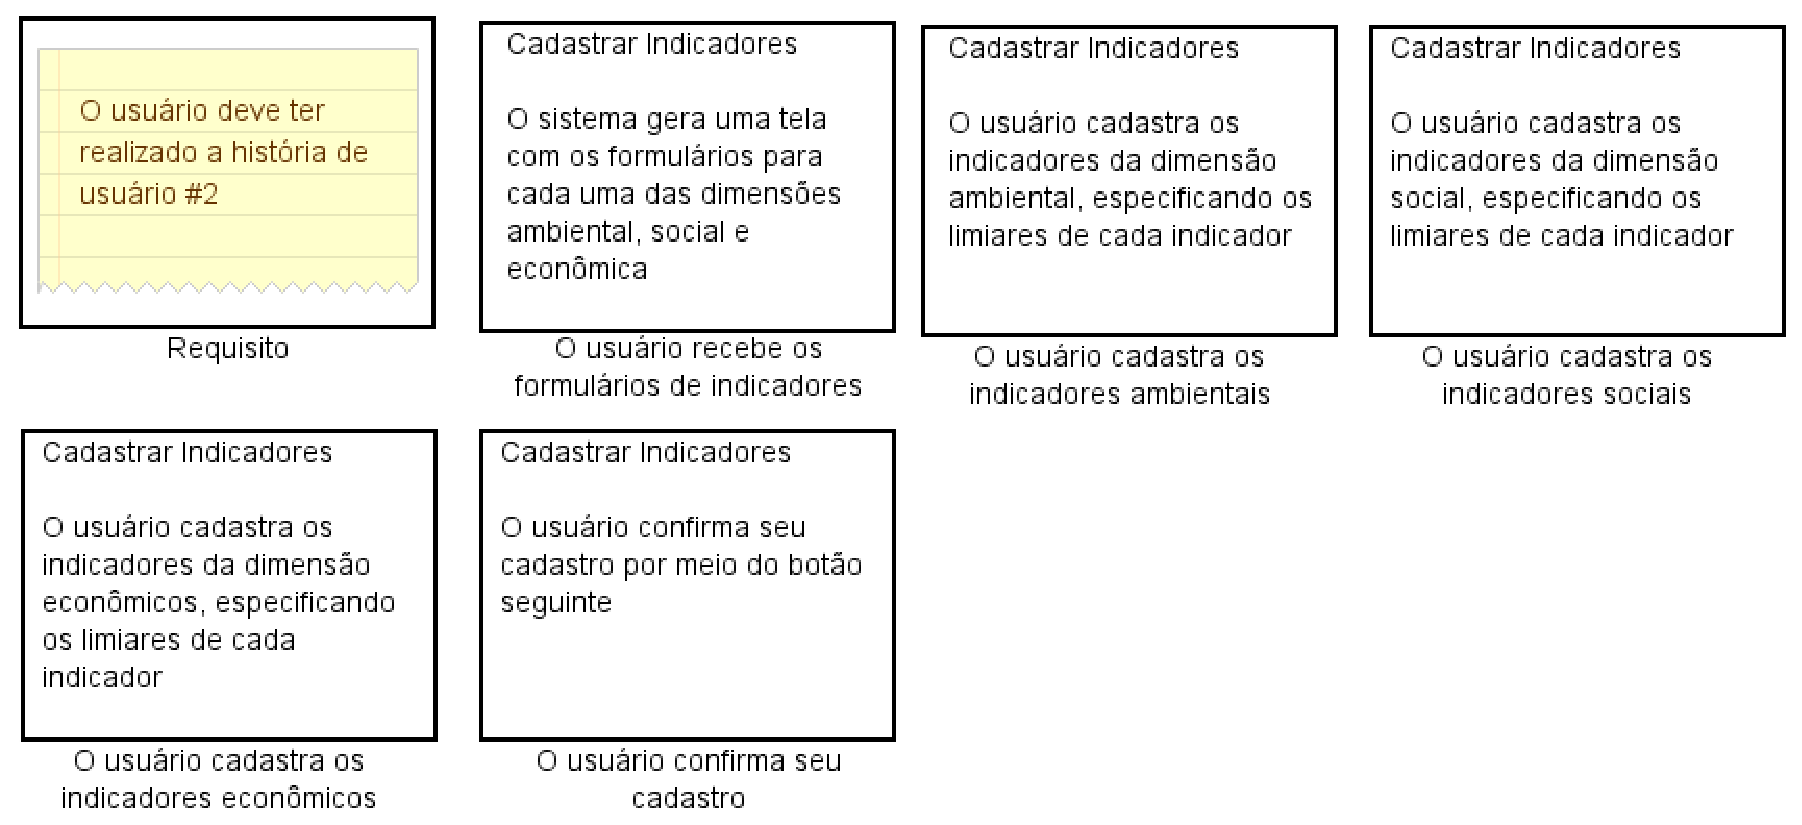
\includegraphics[width=1\columnwidth]{../figures/Story_3}
\par\end{centering}
\begin{centering}
\textit{\small{}StoryBoard 3.}
\par\end{centering}{\small \par}
\centering{}\caption{Storyboards números 1–3.\label{fig:Storyboard-numero-1}}
\end{figure}

\begin{figure}[H]
\begin{centering}
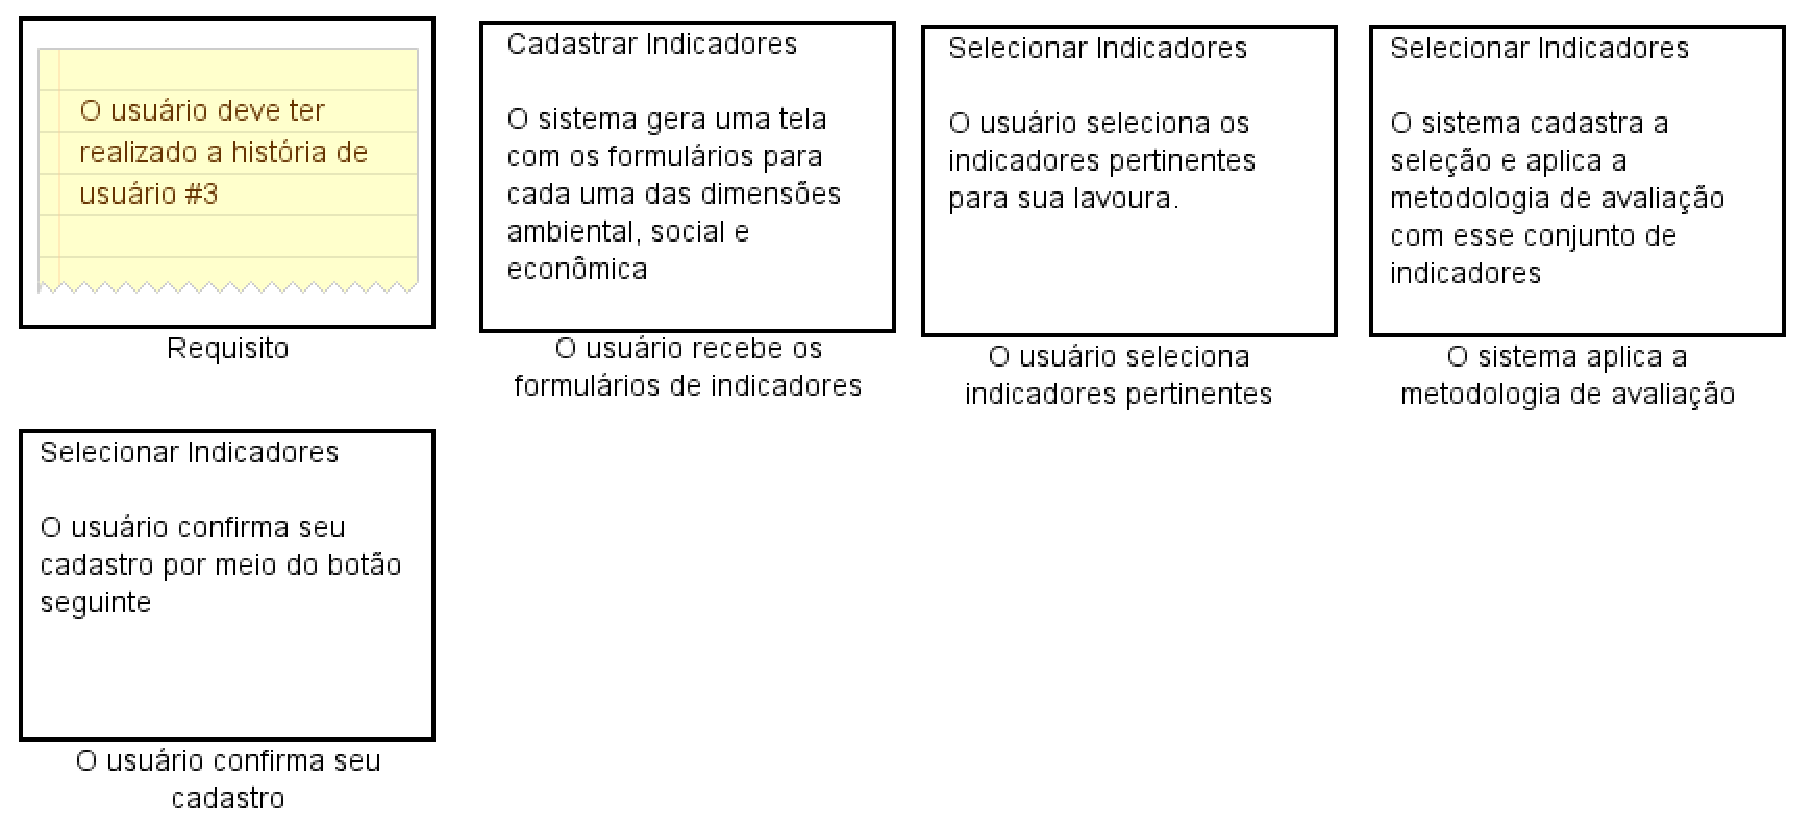
\includegraphics[width=1\columnwidth]{../figures/Story_4}
\par\end{centering}
\begin{centering}
\textit{\small{}StoryBoard 4.}
\par\end{centering}{\small \par}
\bigskip{}

\begin{centering}
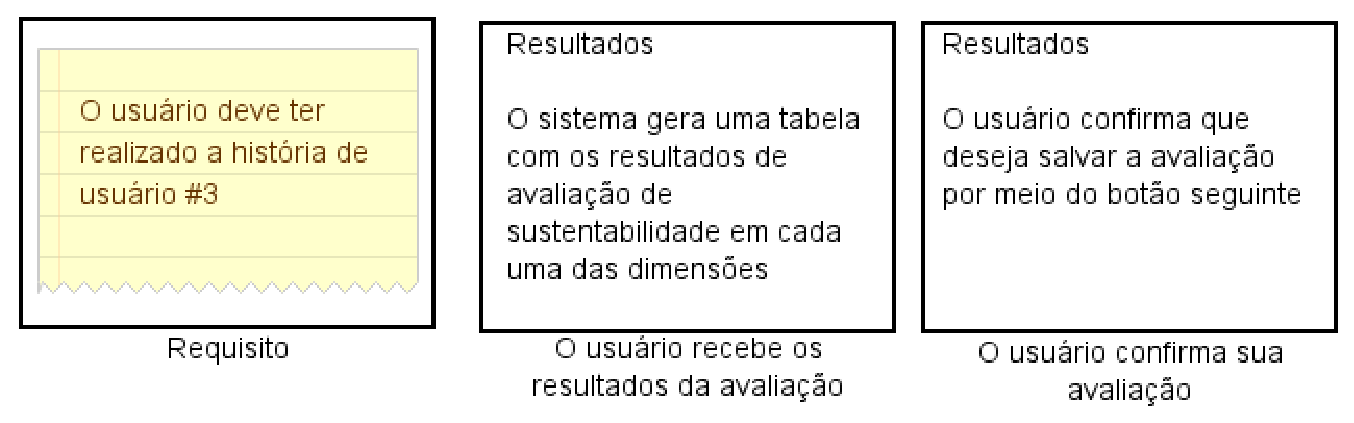
\includegraphics[width=1\columnwidth]{../figures/Story_5}
\par\end{centering}
\begin{centering}
\textit{\small{}StoryBoard 5.}
\par\end{centering}{\small \par}
\bigskip{}

\begin{centering}
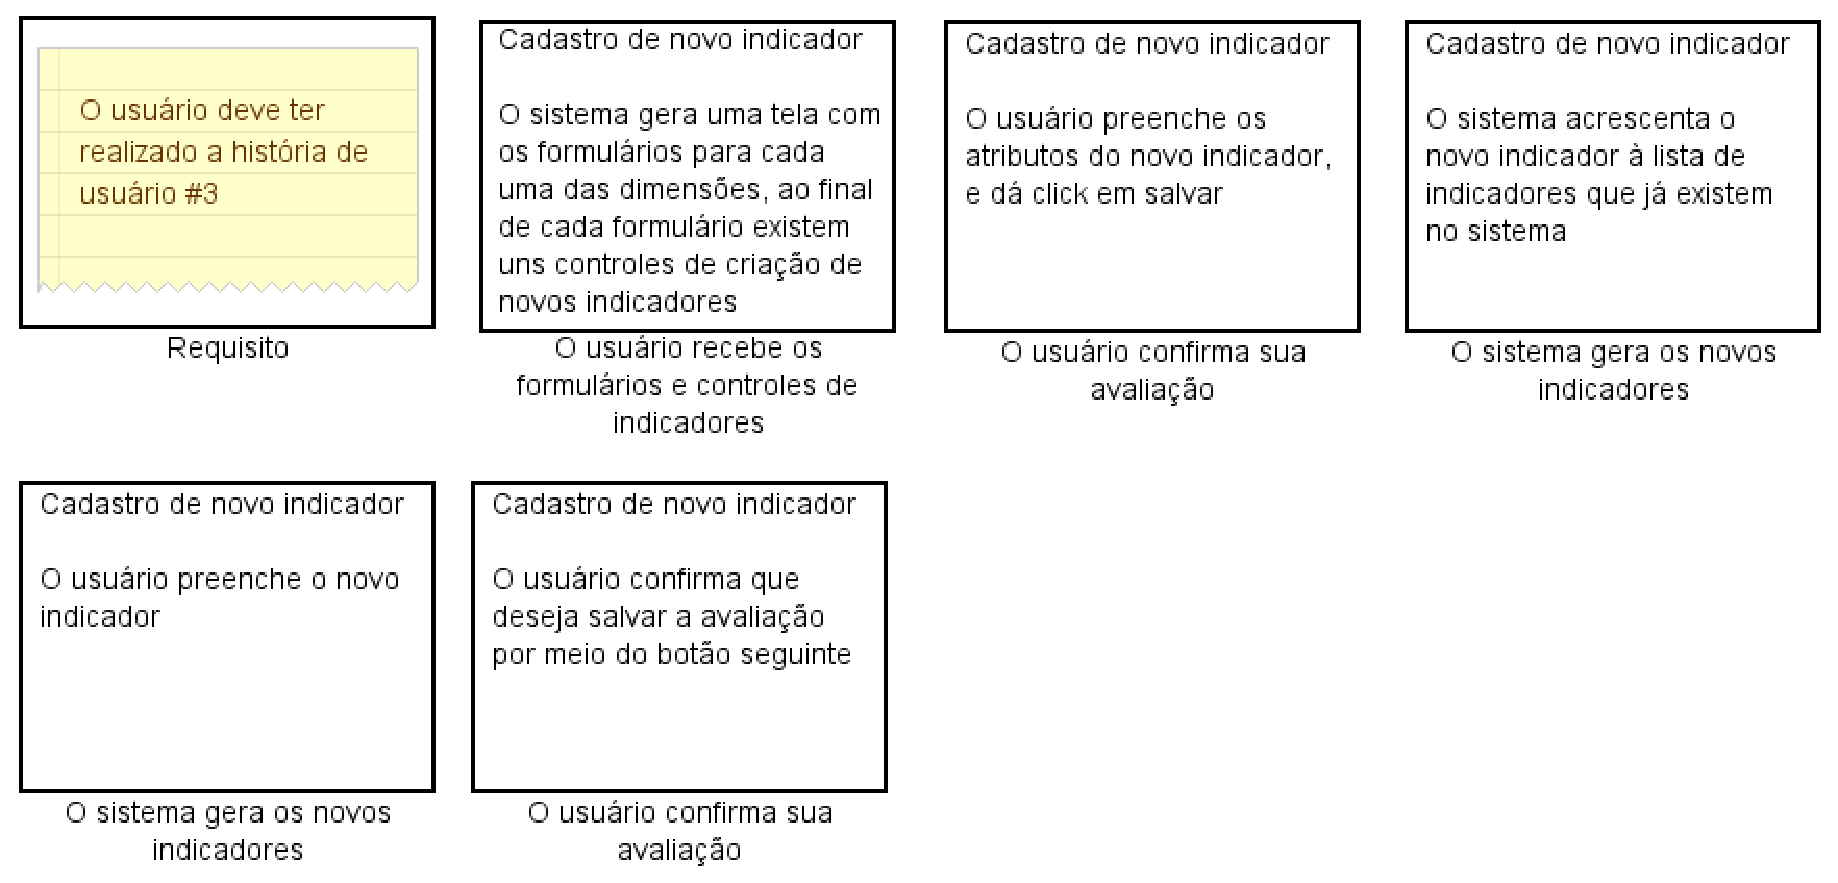
\includegraphics[width=1\columnwidth]{../figures/Story_7}
\par\end{centering}
\begin{centering}
\textit{\small{}StoryBoard 6.}
\par\end{centering}{\small \par}
\bigskip{}

\centering{}\caption{Storyboards números 4–6.\label{fig:Storyboard-numero-4}}
\end{figure}


\section{Mockups das Interfaces do SustenAgro}

Mockups permitem uma representação visual das interfaces do sistema
para ajudar no seu entendimento, fazer demonstrações, avaliações do
design, dentre outros propósitos. As Figuras \ref{fig:Mockup_home}
e \ref{fig:Mockup_indicators} mostram algumas telas com desenhos
dos Mockups que foram avaliados e validados pela equipe do projeto.

\begin{figure}
\centering{}\includegraphics[width=1\columnwidth]{\string"../figures/Mockup Main\string".eps}\caption{Mockup da tela da Home Page do SustenAgro.\label{fig:Mockup_home}}
\end{figure}

\begin{figure}
\centering{}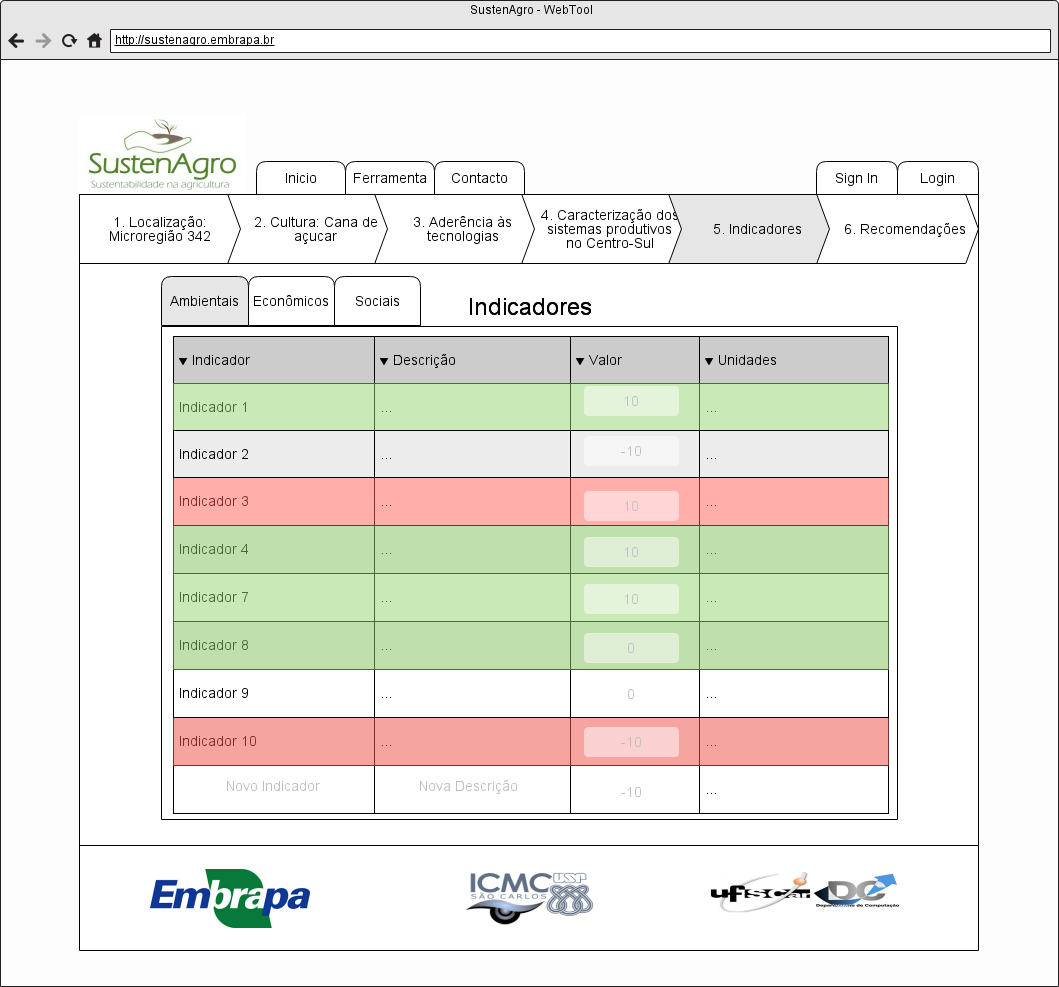
\includegraphics[width=1\columnwidth]{../figures/Tool_environmental_indicators}\caption{Mockup da tela de indicadores do SustenAgro.\label{fig:Mockup_indicators}}
\end{figure}


\section{Protótipo da Interface Gráfica do SustenAgro}

O primeiro protótipo da interface gráfica do SustenAgro está publicado
nos servidores do laboratório Intermídia do ICMC\nobreakdash-USP
\footnote{http://biomac.icmc.usp.br:8080/sustenagro/}, na Figura
\ref{fig:Home} é apresentada a página inicial do protótipo.

\begin{figure}
\begin{centering}
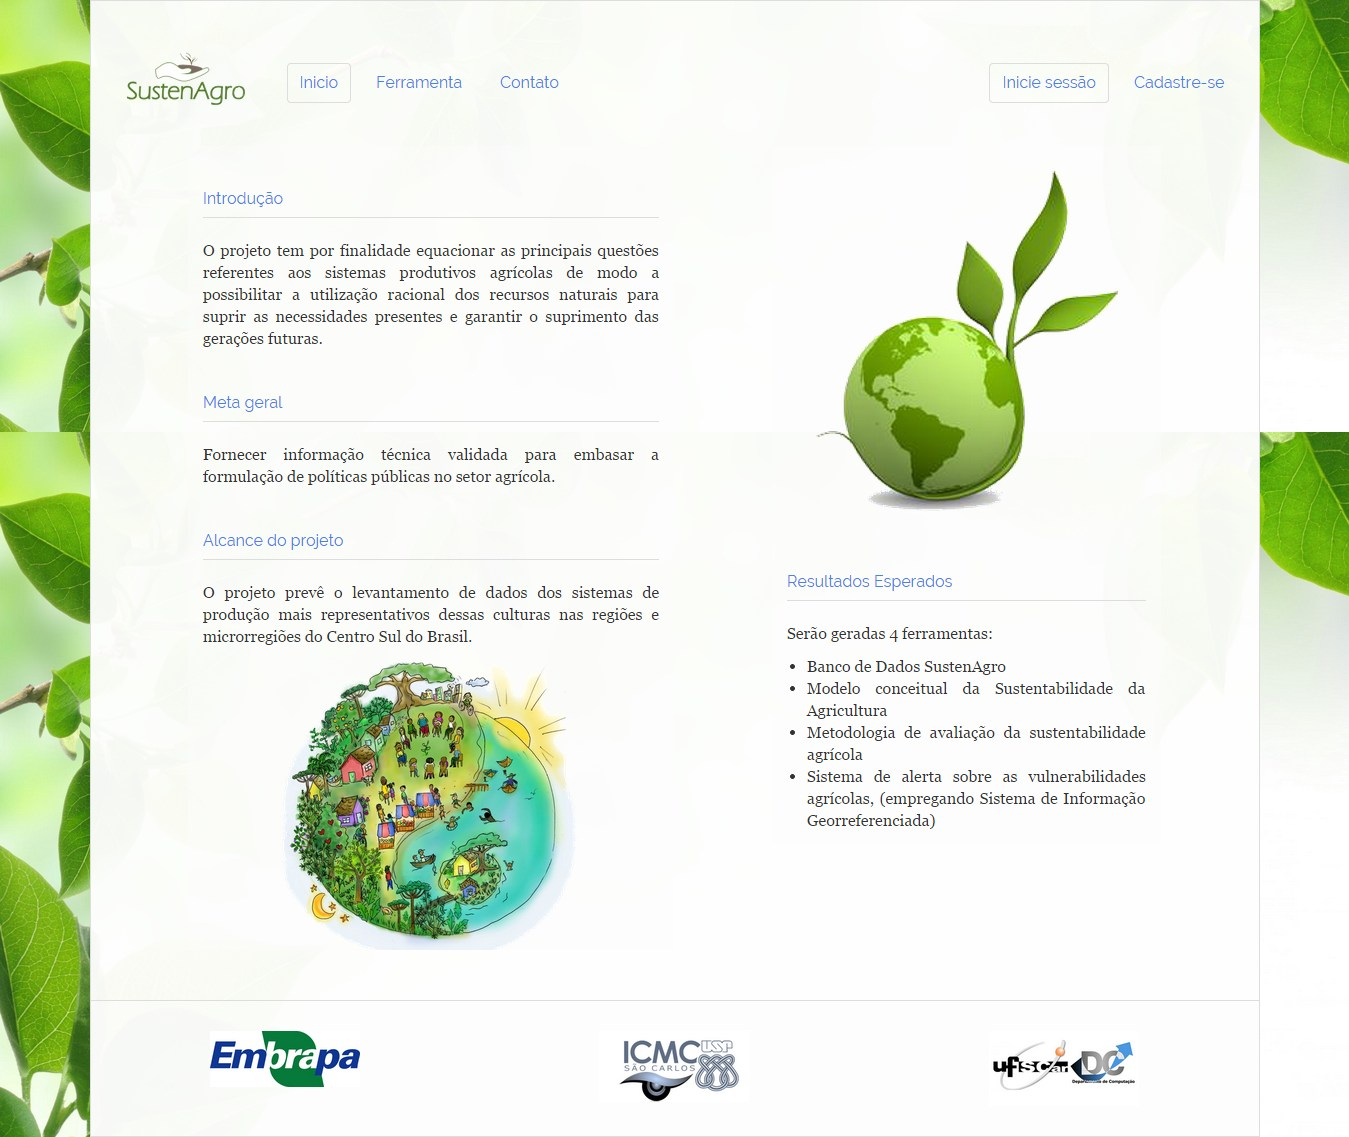
\includegraphics[width=1\textwidth]{../figures/home}
\par\end{centering}
\caption{Protótipo do SustenAgro – Home Page.\label{fig:Home}}
\end{figure}

Nessa tela pode-se observar o texto explicativo da ferramenta e as
abas de ``Início'', ``Ferramenta'' e ``Contato''. O menu da
ferramenta permite iniciar o processo de avaliação de sustentabilidade.

Na Figura \ref{fig:Indicators}, é apresentada a página dos indicadores,
onde se descreve o processo de avaliação. Ele começa com uma descrição
base do processo, a localização geográfica da unidade produtiva, a
caracterização dela, os indicadores e as recomendações que o sistema
vai gerar.

\begin{figure}
\centering{}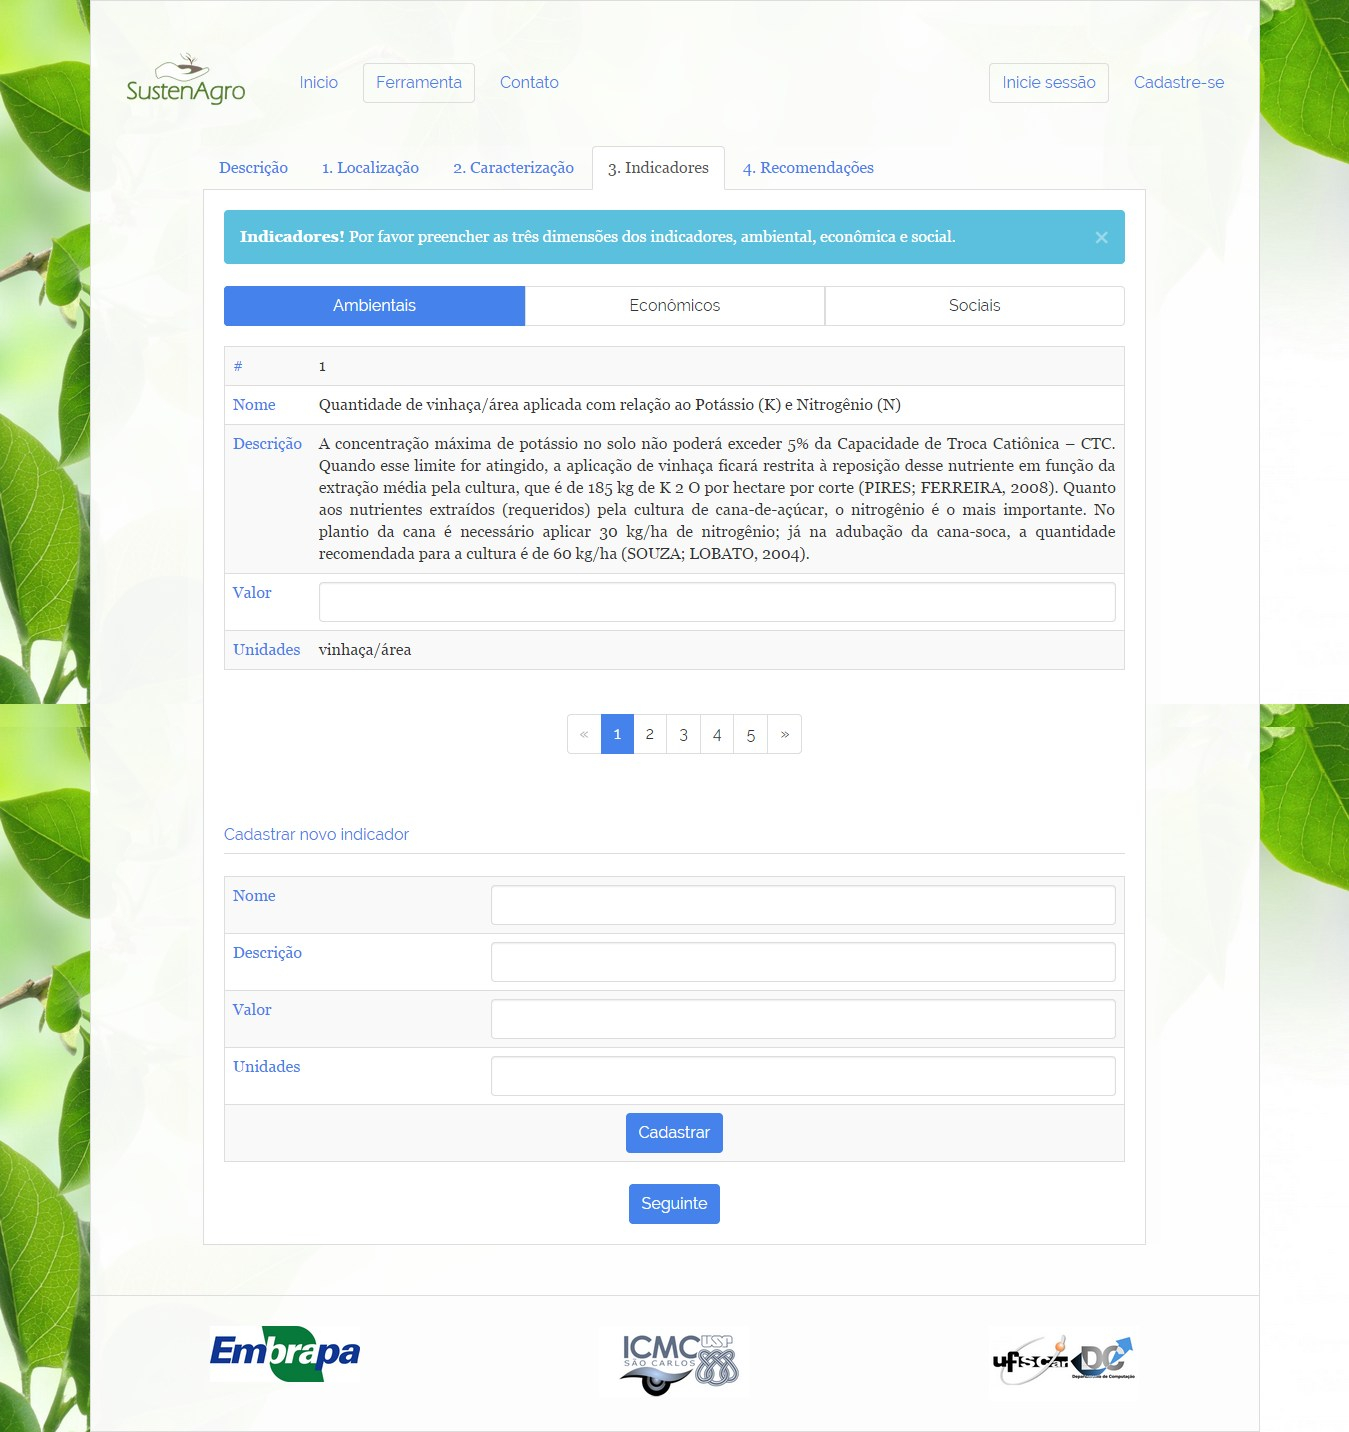
\includegraphics[width=1\columnwidth]{../figures/indicators}\caption{Protótipo do SustenAgro - Indicadores.\label{fig:Indicators}}
\end{figure}


\section{Características do sistema}

Uma vez cadastrada a unidade produtiva/fazenda disponibiliza-se a
opção de criar nova avaliação, ação que vai gerar a tela da figura
9 que permite visualizar as variaveis de eficiencia e os indicadores
para que os usuários preencham cada uma segundo a realidade da unidade
produtiva em avaliação, cada indicador ou variavel de eficiencia tem
varias opções que estão ligadas a valores que quantificam a sustentabilidade,
esses valores estão definidos na ontologia da sustentabilidade e serao
os valores de ingreso para a formula que vai gerar os indices da sustentabilidade. 

\begin{figure}
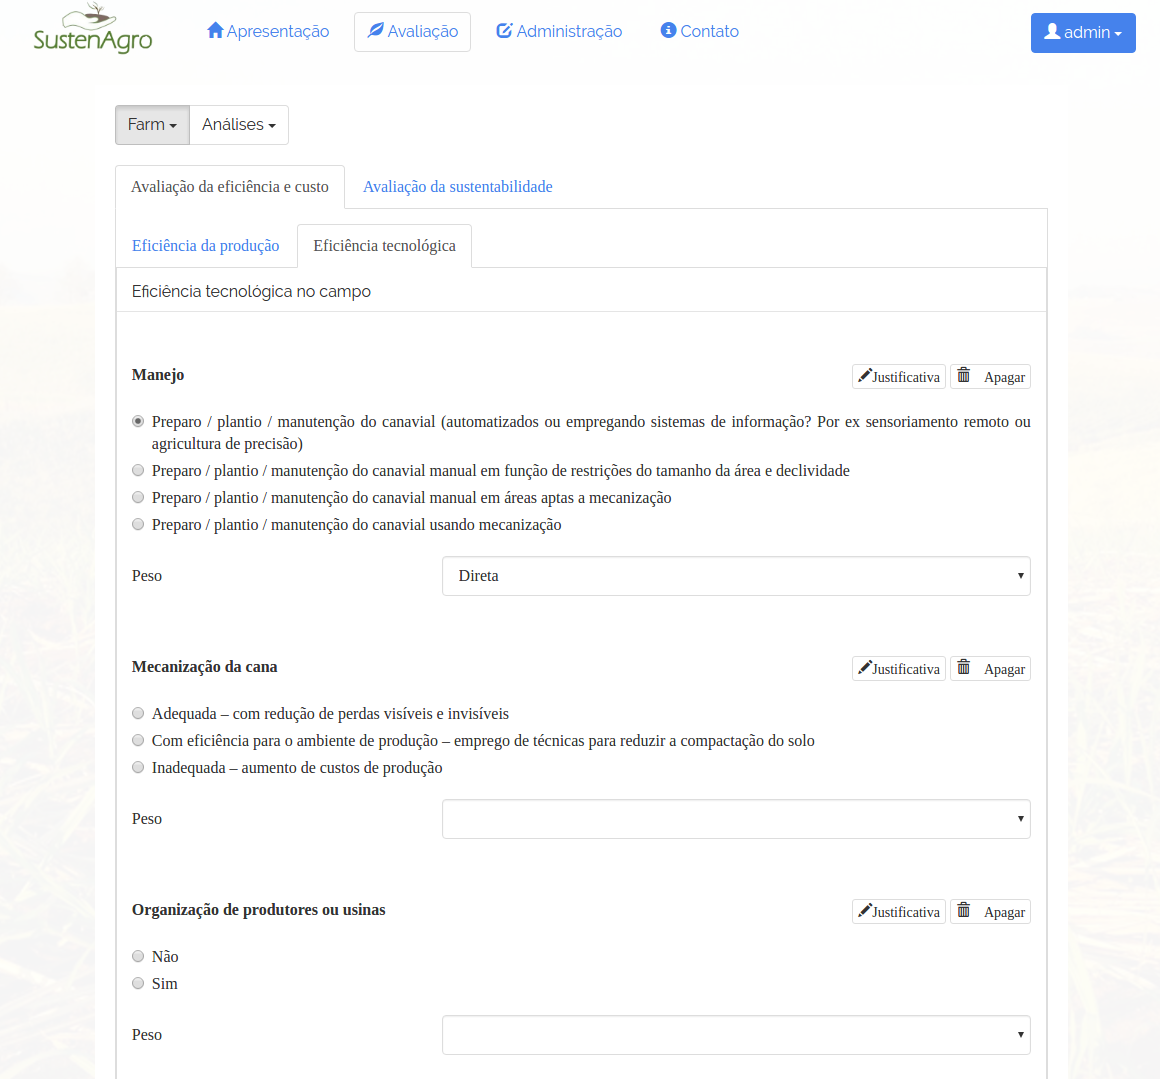
\includegraphics[scale=0.5]{../figures/SustenAgro-scenario}

\caption{Cadastro das variaveis/indicadores}
\end{figure}

A partir desses desses dados cadastrados são gerados os resultados
do sistema que consistem na planilha de ediciência e custo, na planilha
da sustentabilidade e o relatorio do sistema, as planilhas permitem
a visualizar os atributos das variaveis de eficiência e dos indicadores
e a tela de relatorio que apresenta a matrix de avaliação onde são
relaciondas as variaveis de eficiência e de sustentabilidade, o relatio
é apresentado na figura 10. 

\begin{figure}
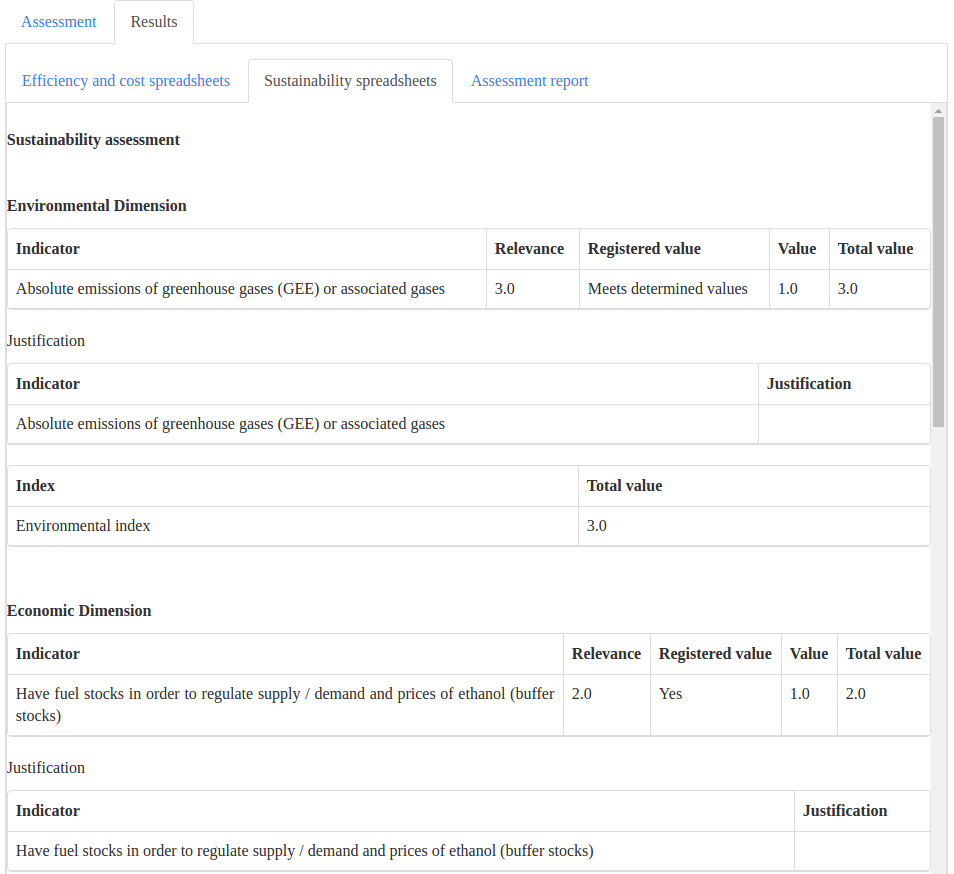
\includegraphics{../figures/SustenAgro-results}

\caption{Formato das planilhas de resultado}
\end{figure}


\section{Considerações Finais}

O desenvolvimento do sistema Sustenagro satisfaz uma necessidade presente
na unidade da Embrapa Meio Ambiente: um sistema de avaliação de sustentabilidade
em sistemas produtivos de cana-de-açúcar. Ele permitirá adquirir dados
do estado atual de sustentabilidade nas fazendas e usinas e assim
embasar e formalizar políticas publicas para promover práticas produtivas
mais sustentáveis de acordo com critérios ambientais, sociais e econômicos.

Além de satisfazer uma necessidade institucional, o SustenAgro se
consolida como uma proposta de SAD baseado em conhecimento e vinculado
às tecnologias da web semântica, um processo que requer um trabalho
de pesquisa e de inovação tecnológica. A pesquisa deste trabalho de
mestrado, usará o SustenAgro como uma base de testes realista para
os conceitos e ferramentas desenvolvidos. 

Após o desenvolvimento do Sistema SustenAgro, poder-se-a analisar
as características fundamentais desse tipo de SAD e tentar reusar
a arquitetura em outros SADs da própria Embrapa.
\end{document}
